% autosam.tex
% Annotated sample file for the preparation of LaTeX files
% for the final versions of papers submitted to or accepted for 
% publication in AUTOMATICA.

% See also the Information for Authors.

% Make sure that the zip file that you send contains all the 
% files, including the files for the figures and the bib file.

% Output produced with the elsart style file does not imitate the
% AUTOMATICA style. The style file is generic for all Elsevier
% journals and the output is laid out for easy copy editing. The
% final document is produced from the source file in the
% AUTOMATICA style at Elsevier.

% You may use the style file autart.cls to obtain a two-column 
% document (see below) that more or less imitates the printed 
% Automatica style. This may helpful to improve the formatting 
% of the equations, tables and figures, and also serves to check 
% whether the paper satisfies the length requirements.

% Please note: Authors must not create their own macros.

% For further information regarding the preparation of LaTeX files 
% for Elsevier, please refer to the "Full Instructions to Authors" 
% from Elsevier's anonymous ftp server on ftp.elsevier.nl in the
% directory pub/styles, or from the internet (CTAN sites) on
% ftp.shsu.edu, ftp.dante.de and ftp.tex.ac.uk in the directory
% tex-archive/macros/latex/contrib/supported/elsevier.


%\documentclass{elsart}               % The use of LaTeX2e is preferred.

\documentclass[twocolumn]{autart}    % Enable this line and disable the 
                                     % preceding line to obtain a two-column 
                                     % document whose style resembles the
                                     % printed Automatica style.

\usepackage{graphicx}
\usepackage{color}
\usepackage{amssymb}
\usepackage{amsmath}
\setcounter{tocdepth}{3}
\usepackage{graphicx}
\usepackage{tikz}
\usepackage{pgfplots}
\usepackage{framed}
\usepackage{listings}
\usepackage{algorithm,algpseudocode}
\usepackage{epstopdf}
\usepackage{cite}
\usepackage{pifont}
\usepackage{inconsolata}
\usepackage{todonotes}
\usetikzlibrary{positioning, automata, shapes.arrows, calc, shapes, arrows}
\usetikzlibrary{patterns}

\tikzset{
    %Define style for boxes
    box/.style={
           rectangle,
           rounded corners,
           draw=black, very thick,
           fill=yellow!20,
           text width=10em,
           minimum height=2em,
           text centered},
 % 
  futurebox/.style={
           rectangle,
           rounded corners,
           draw=black, very thick,
           fill=blue!10,
           text width=10em,
           minimum height=2em,
           text centered},
 % 
  longfuturebox/.style={
           rectangle,
           rounded corners,
           draw=black, very thick,
           fill=purple!20,
           text width=10em,
           minimum height=2em,
           text centered},
%
    % Define arrow style
    arrow/.style={
           ->,
           thick,
           shorten <=2pt,
           shorten >=2pt,}
}

\usepackage{url}

%\newcommand{\tool}{{\sf DSSynth}\xspace}
\newcommand{\addtodo}[1]{\textcolor{red}{[#1]}}
\newcommand{\mat}[1]{{#1}}
\renewcommand{\vec}[1]{{#1}}
\newcommand{\comment}[1]{}
\newtheorem{lemma}{Lemma}
\newtheorem{theorem}{Theorem}
\newtheorem{corollary}{Corollary}
\newtheorem{proof}{Proof}

\newcommand{\xmark}{\ding{55}}

\renewcommand{\note}[1]{\textcolor{red}{[#1]}}
\newcommand{\reply}[1]{\textcolor{blue}{[#1]}}

\begin{document}
\newcommand\tool{{\sf DSSynth}}
\begin{frontmatter}

%\runtitle{Insert a suggested running title}  % Running title for regular 
                                              % papers but only if the title  
                                              % is over 5 words. Running title 
                                              % is not shown in output.

%\thanksref{footnoteinfo}

\title{Automated Formal Synthesis\\ 
of Safe Digital Controllers 
for Continuous Plants}
% Title, preferably not more
% than 10 words.

%\thanks[footnoteinfo]{This paper was not presented at any IFAC 
%meeting. Corresponding author M.~T.~Cicero. Tel. +XXXIX-VI-mmmxxi. 
%Fax +XXXIX-VI-mmmxxv.}

\author[oxford]{Alessandro Abate}\ead{alessandro.abate@cs.ox.ac.uk},
\author[manaus]{Iury Bessa}\ead{iurybessa@ufam.edu.br},
\author[oxford]{Dario Cattaruzza}\ead{dario.cattaruzza@cs.ox.ac.uk},
\author[manchester]{Lucas Cordeiro}\ead{lucas.cordeiro@manchester.ac.uk},
\author[cambridge]{Cristina David}\ead{cd652@cam.ac.uk},
\author[oxford]{Pascal Kessel}\ead{pascal.kesseli@cs.ox.ac.uk},
\author[oxford]{Daniel Kroening}\ead{kroening@cs.ox.ac.uk},
\author[oxford]{Elizabeth Polgreen}\ead{elizabeth.polgreen@cs.ox.ac.uk}

\address[oxford]{University of Oxford, UK}
\address[cambridge]{University of Cambridge, UK}
\address[manchester]{University of Manchester, UK}
\address[manaus]{Federal University of Amazonas, Brazil} 
          
\begin{keyword}                           % Five to ten keywords,  
Digital control synthesis; Safety requirements; Analog/Digital conversion; Quantization errors; Time sampling.               % chosen from the IFAC 
\end{keyword}                             % keyword list or with the 
                                          % help of the Automatica 
                                          % keyword wizard

%\keywords{
%State-space dynamical models of physical systems; 
%digital controllers; 
%analogue-to-digital converters; 
%time sampling; 
%quantization; 
%fixed-point arithmetic; 
%CEGIS; 
%safety requirements. 
%}


\begin{abstract}                          % Abstract of not more than 200 words.
%\textcolor{red}{Cristina: Can you please write an initial version of the abstract.}
We present a sound and automated approach to synthesizing safe,
digital controllers for physical plants represented as linear,
time-invariant models. Models are defined as differential equations
with inputs, evolving over a continuous state space. The synthesis
accounts for errors caused by the digitization effects introduced by
the controller. Our approach uses counterexample-guided inductive
synthesis (CEGIS): an inductive generalisation phase produces a
possible solution that is known to stabilize the system but that may
not be safe for all initial conditions. 
\ifx\axelerator
Safety is then verified either
via Bounded Model Checking or abstract acceleration;
\else
Safety is then verified via Bounded Model Checking;
\fi 
if the verification step fails, a
counterexample is provided to the inductive generalisation and the
process iterates until a safe controller is obtained.  We demonstrate
the practical value of this approach by automatically synthesizing
safe controllers for physical plant models from the digital control
literature.
\end{abstract}

\end{frontmatter}

\section{Introduction}

Modern implementations of embedded control systems have proliferated
with the availability of low-cost devices that can perform highly
non-trivial control tasks, with significant impact in numerous
application areas such as the life sciences, high-precision control, 
automotive and robotics~\cite{astrom1997computer, Franklin15}.  
Provably correct synthesis of control software for such platforms is non-trivial, 
even in cases with unsophisticated dynamics. 

In this paper, we examine the case of Linear Time Invariant (LTI)
models, for which the synthesis of controllers is well understood.
However, the use of digital control architectures adds new challenges
caused by artefacts specific to digital control, such as the effects
of finite-precision arithmetic, time discretization and quantization
errors introduced by A/D and D/A conversion.
%
Given an LTI model, we develop an automatic technique for generating
correct-by-construction digital controllers that addresses all these
challenges. Specifically, we automatically synthesize %stable and 
safe,
software-implemented embedded controllers.  
%Due to the complexity of
%such closed-loop systems, we focus on linear models with known
%configurations, and perform parametric synthesis of controllers.
%meeting a number of properties that define their desired behavior.

%% While research on digital control is well developed~\cite{astrom1997computer},
%% automated and sound control synthesis is challenging, particularly when the
%% synthesis objective goes beyond classical stability.  There are recent methods
%% for verifying reachability properties of a given controller~\cite{FLD+11}.
%% However, these methods have not been generalized to control synthesis.  
%% Note that a synthesis algorithm that guarantees stability does not
%% ensure safety: the system might transitively visit an unsafe state resulting
%% in unrecoverable failure. %% Programming expertise is a key
%% barrier to broad adoption of correct digital controllers, and requires
%% considerable knowledge outside of the expertise of many control engineers.

%% Beyond classical a-posteriori validation in digital control, there has been
%% plenty of previous work aiming at \emph{verifying} a given designed
%% controller, which however broadly lack automation.  Recent work has studied
%% the stability of digital controllers considering implementation aspects,
%% i.e., fixed-point arithmetic and the word length~\cite{Bessa16}.  They
%% exploit advances in bit-accurate verification of C programs to obtain a
%% verifier for software-implemented digital control.


%% we leverage a very recent step-change in the automation and
%% scalability of \emph{program synthesis}.  %% Program synthesis engines use a
%% %% specification as the starting point, and subsequently generate a sequence of
%% %% candidate programs from a given template.  The candidate programs are
%% %% iteratively refined to eventually satisfy the specification.
%% Program
%% synthesizers implementing Counter-Example Guided Inductive Synthesis
%% (CEGIS)~\cite{DBLP:conf/asplos/Solar-LezamaTBSS06} are now able to generate
%% programs for highly non-trivial specifications with a very high degree of
%% automation.  Modern synthesis engines combine automated testing, genetic
%% algorithms, and SMT-based automated
%% reasoning~\cite{DBLP:journals/corr/AlurFSS16a, DBLP:conf/lpar/DavidKL15}.

%% By combining state-of-the-art synthesis engines we present a tool that
%% automatically generates digital controllers for a given continuous plant
%% model that are correct by construction.  This approach delivers a high
%% degree of automation, promises to reduce the cost and time of development of
%% digital control dramatically, and requires considerably less expertise than
%% a-posteriori verification.  Specifically, we synthesize stable,
%% software-implemented embedded controllers along with a model of a physical
%% plant.  Due to the complexity of such closed-loop systems, in this work we
%% focus on linear models with known configurations, and perform parametric
%% synthesis of stabilizing digital controllers with a number of properties that
%% define their desired behaviour.

Our work addresses challenging aspects of the control synthesis problem:  
we perform digital control synthesis over a ``hybrid model'',
namely a model encompassing a plant exhibiting continuous behavior, 
whereas the controller operates in discrete time and over a quantized domain.  
In particular, our model evaluates the effects of the quantizers (A/D and D/A
converters), as well as representation
errors introduced by the controller working  %% artifacts such as an
%% observer~\cite{astrom1997computer}
in a finite-precision domain. Our model also accounts for representation errors introduced
by our modelling of the plant using finite precision arithmetic. 
We reason safety requirements, which are frequently overlooked in conventional feedback control synthesis, but
play a key role in systems engineering, particularly for safety-critical applications of clear concern in modern autonomy contexts.  

%% Using state of the art verifiers, we evaluate these models against
%% automatically synthesised controllers using CEGIS-based synsthesis that
%% incorporate the above mentioned artifacts in different models of
%% Single-Input/Single-Output (SISO) systems.
\ifx\axelerator
In this paper we present two novel approaches for the synthesis of
digital controllers, both of which make 
\else
In this paper we present a novel approach for the synthesis of digital controllers,
making 
\fi
use of the framework known as counterexample guided
inductive synthesis (CEGIS)~\cite{jha-icse10,
  DBLP:conf/asplos/Solar-LezamaTBSS06}, 
  a technique from formal methods that has recently shown much promise and which we 
  export in this work to a control-theoretical setup.  
CEGIS is an iterative process, where each iteration performs inductive
generalisation based on counterexamples provided by a verification
oracle (see Section~\ref{ssec:cegis}). The inductive generalisation uses information 
about a limited number of inputs to compute a candidate solution
for the entire range of possible inputs. Our two instantiations of CEGIS are described next.

%% offer three modes of
%% operation that address different aspects of the problem.
%% {\em The first  approach} uses a transfer-function based analysis that
%% solves the problem of robust stability for closed loop systems for a
%% collection of unstable plants.  Inthis case, there is no safety
%% specification since we are working in the frequency domain.
\ifx\axelerator
\emph{The first approach} 
\else
Our approach
\fi
uses a multi-staged technique that starts by devising a
digital controller that stabilizes the plant model while remaining safe for a
pre-selected time horizon and a single initial state; then, it verifies
unbounded-time safety by unfolding the model dynamics, considering the 
full set of initial states, and checking a \emph{completeness
threshold}~\cite{DBLP:conf/vmcai/KroeningS03}, i.e., the number of
iterations required to sufficiently unwind the closed-loop state-space
model such that the safety boundaries are not violated for any larger number of
iterations.  

\ifx\axelerator
Instead of unfolding the dynamics, \emph{the second approach}
employs \emph{abstract acceleration}~\cite{cattaruzza2015unbounded} to
evaluate all possible progressions of the model simultaneously. 
Additionally, this approach uses the \emph{abstraction-refinement} template \cite{DBLP:conf/cav/ClarkeGJLV00},
enabling one to start with a very simple (abstract) description of the model 
regardless of the complexity of its dynamics, and to refine to more complex models only 
when a solution cannot be found.
\fi

We provide experimental results showing that we are able to
efficiently synthesize safe controllers for a set of intricate physical
plant models taken from the digital control literature.
%\addtodo{add more here once we have the experimental results ready}

%% \addtodo{CD: the novelty compared to CAV'17 needs to be clarified}
This paper is an extension of~\cite{DBLP:conf/cav/AbateBCCDKKP17}
and makes the following contributions (the fourth is a 
specific extension to~\cite{DBLP:conf/cav/AbateBCCDKKP17}): 
%
\begin{enumerate}

  % Additions from CAV:
  % continuous time
  % floating point 
\item We automatically generate \emph{correct-by-construction} digital
  controllers using an inductive synthesis approach (CEGIS).  
  %% This application is non-trivial and addresses challenges specific to digital control
  %% systems, such as the presence of A/D quantizers and FWL operations.  
  In addition a stability property, the automatically computed state-feedback
  controllers must also guarantee a given safety specification.
  The implication is that, as opposed to existing
  methods for controller synthesis which rely on transfer function
  representations, we must consider a state-space representation of
  the physical system. Such a representation requires ensuring the
  specification over actual traces of the model, alongside the
  numerical soundness required by the effects of discretisation and
  finite-precision errors.

  
%%   \note{[this statement is way too broad] Existing methods for controller synthesis rely on transfer 
%%   function representations, which are inadequate to prove safety requirements. } 
%% %
\ifx\axelerator
\item We provide two novel algorithms: the first, a multi-staged approach, relies on 
  an unfolding of the dynamics up to a completeness threshold, while the
  second one is abstraction-based and leverages abstraction/refinement and
  acceleration to improve scalability while retaining soundness.  %% A third
  %% algorithm evaluates systems using transfer functions where no state-space
  %% description is given.
  Both approaches provide sound synthesis of 
  feedback controllers and consider the various sources of imprecision in
  the implementation of the control algorithm and in the modeling of the
  plant. 
\else  
\item We present a novel multi-staged approach to synthesising digital controllers, using on 
  an unfolding of the dynamics up to a completeness threshold, and bit precise Bounded Model
  Checking to account for sources of imprecision in the implementation of the digital control algorithm
  and the modelling of the plant.
  \fi
  
%
\item We develop a model for different sources of quantization error and account for 
  their effect on safety.  We provide bounds that ensure the
  safety of our controllers in a hybrid (i.e., continuous/digital) domain.


%\item While~\cite{DBLP:conf/cav/AbateBCCDKKP17} is restricted to models in discrete 
%time, \note{in the current paper we present an approach for
%  soundly evaluating safety in combined continuous-discrete time and space. [this is via the AA-based back-end. However this part is not in the experiments, afaik.]}

\item A limitation of the work in~\cite{DBLP:conf/cav/AbateBCCDKKP17} 
  is its restriction to fixed-point arithmetic, meaning that fixed-point
  numbers are employed for the representation of both the plant and the
  controller, as well as for the operations performed by each of them. 
  Conversely, in the current paper we also make use of floating-point
  arithmetic.  
  %\note{Additionally, we enhance the
  %implementation with an SMT back-end, allowing us to also use reals in order
  %to represent the states of the plant.} 
  
\end{enumerate}
  
%-------------------------------
\section{Related Work}
\label{sec:relw}
%-------------------------------

\textbf{CEGIS --} Program synthesis is the problem of computing
correct-by-design programs from high-level specifications. Algorithms
for this problem have made substantial progress in recent years, in
particular CEGIS, which is a recent approach to inductive synthesis.
%% borrowing ideas from counterexample guided abstraction refinement
%% (CEGAR)~\cite{DBLP:conf/cav/ClarkeGJLV00} and
%% superoptimisation~\cite{DBLP:conf/iclp/BrainCVF06,
%%   DBLP:conf/asplosss/Massalin87}.  
%% \note{might be confusing that we relate the CEGAR architecture also to Abstract Acceleration?}   
%% This approach uses an iterative
%% process (see Section~\ref{ssec:cegis}), where each iteration performs inductive generalisation based
%% on counterexamples provided by a verification oracle.  In the absence
%% of complete specifications, oracles are queried to distinguish between
%% non-equivalent
%% programs~\cite{jha-icse10,DBLP:conf/fmcad/AlurBJMRSSSTU13}.

%% for instance~\cite{itzhaky2010simple} 
%% to inductively synthesize invariants for the generation of desired programs.

Program synthesizers are an ideal fit for the synthesis of digital controllers, since
the semantics of programs precisely capture the effects of finite-precision arithmetic.  
In~\cite{DBLP:conf/cdc/RavanbakhshS15}, the authors use CEGIS 
for the synthesis of switching controllers for stabilizing continuous-time
plants with polynomial dynamics.  The work extends to affine systems, but is
limited by the capacity of the state-of-the-art SMT solvers for solving
linear arithmetic.  Since this approach uses switching models instead of
linear dynamics for the digital controller, it avoids problems related to
finite precision arithmetic, but potentially suffers from state-space
explosion.  Moreover, in \cite{DBLP:conf/emsoft/RavanbakhshS16} the same
authors use a CEGIS-based approach for synthesizing continuous-time
switching controllers that guarantee \emph{reach-while-stay} properties of
closed-loop systems, i.e., properties that specify a set of goal states and
safe states (constrained reachability).  This solution is based on
synthesizing control Lyapunov functions for switched systems that yield
switching controllers with a guaranteed minimum dwell time in each mode. 
However, both approaches are unsuitable for the kind of controllers that we seek to
synthesize.

The work in~\cite{hscc-paper} synthesizes stabilizing controllers for
continuous plants given as transfer functions by exploiting bit-accurate
verification of software-implemented digital controllers~\cite{Bessa16}. 
While this work also uses CEGIS, the approach is restricted to digital
controllers for stable closed-loop systems given as transfer function
models: this results in a static check on their coefficients.  By contrast,
in the current paper we consider a state-space representation of the
physical system, which requires ensuring the specification over actual
traces of the model, alongside the numerical soundness required by the
effects of discretisation and finite-precision errors.

A~state-space model has known advantages over the transfer function
representation~\cite{Franklin15}, as 
% it naturally generalizes to multivariate systems (i.e., with multiple inputs and outputs); and 
it allows synthesis of controllers with guarantees on the internal dynamics, e.g., 
%to synthesize controllers that make the closed-loop model 
\emph{safety}.  Our work indeed focuses on the safety of internal states, 
which is by and large overlooked in the standard (digital) control literature, 
by default focussed on stability properties.  
Moreover, our work integrates an abstraction-refinement (CEGAR) step inside the main CEGIS loop.

The technique underpinning tools such as Pessoa~\cite{mazo2010pessoa} and related extensions \cite{Anta2010,liu16} and applications \cite{zamani2014}, 
synthesizes correct-by-design embedded control software for LTI models.    
It is based on the abstraction of the model to a finite-state machine, 
and on the formal control synthesis over safety- and reachability-based temporal properties thereon.  
%Based on this safety specification, \mbox{Pessoa} can synthesize embedded controller software for a range of
%properties.  
The controller software can then be refined (implemented) over the concrete LTI model. 
%can be more complicated than
%the state-feedback control we synthesize, and the properties available cover more detail.  
However, relying on state-space discretization \mbox{Pessoa} is likely to incur in scalability limitations.   
%Along this research line, \cite{Anta2010,liu16} studies the synthesis of digital controllers for
%continuous dynamics, and \cite{zamani2014} extends the approach to the Network Control Systems setup. 

\textbf{Discretization Effects in Control Design --}
Classical work in control synthesis has often disregarded digitalization effects.
Recent results in digital control, however, have focused on separate aspects of discretization, 
including delayed response~\cite{Duggirala2015} and finite word length (FWL) semantics, 
with the goal either to verify~\cite{daes20161} the correctness of the implementation or to optimize~\cite{oudjida2014design} the design.

There are two different problems that arise from FWL semantics.  The first
is the error caused by the inability to represent the exact
state of the physical system, while the second relates to rounding and
saturation errors during mathematical operations.  
In~\cite{fialho1994stability}, a stability measure based on the error of the digital dynamics ensures that
the deviation introduced by FWL does not lead to instability.  
\cite{DBLP:journals/automatica/WuLCC09} uses $\mu$-calculus to directly model the digital controller so that selected
parameters result by design in stable dynamics.  
The analyses in~\cite{DBLP:conf/hybrid/RouxJG15, DBLP:conf/hybrid/WangGRJF16} rely on an
invariant computation on the discrete dynamics using Semi-Definite
Programming (SDP):  while the former contribution uses bounded-input and bounded-output
(BIBO) properties to determine stability, the latter uses Lyapunov-based
quadratic invariants.  In both cases, the SDP solver uses floating-point
arithmetic and soundness is checked by bounding the error.  
An alternative is~\cite{park2016scalable}, where the verification of given control code is
performed against a known model by extracting an LTI model of the code by
symbolic execution: to account for rounding errors, an upper bound is
introduced in the verification phase.  
The work in~\cite{picasso2003stabilization} introduces invariant sets as a mechanism to
bound the quantization error effect on stabilization.  
% as an invariant set that always converges toward the controllable set.  
Similarly, 
\cite{liberzon2003hybrid} evaluates the quantization error dynamics and \note{[unclear] bounds its trajectory to a known region over a finite time period}.   
%This technique works for both linear and non-linear systems.

%\note{Add note explaining relationship of this work with previously published papers. }

%-------------------------------
\section{Preliminaries}
%\label{sec:preliminaries}
\label{sec:model}
%-------------------------------

%-------------------------------
%\subsection{State-space representations of LTI models}
%\label{sec:model}
%-------------------------------

%% A dynamical system is a system in which a function describes the progression
%% of a state over time.  In a continuous domain with linear dynamics, it is
%% described by a first order Ordinary Differential Equation (ODE).
%% \begin{equation}
%% \dot{x}(t)=\mat{A}\vec{x}(t)+\mat{B}\vec{u}(t)% +\vec{w}(t)
%% \label{eq:dynamical}
%% \end{equation}

%-------------------------------
\subsection{State-space representation of physical systems}
\label{sec:model}
%-------------------------------

\begin{figure*}[htb]
\centering

\tikzset{add/.style n args={4}{
    minimum width=6mm,
    path picture={
        \draw[circle] 
            (path picture bounding box.south east) -- (path picture bounding box.north west)
            (path picture bounding box.south west) -- (path picture bounding box.north east);
        \node[draw=none] at ($(path picture bounding box.south)+(0,0.13)$)     {\small #1};
        \node[draw=none] at ($(path picture bounding box.west)+(0.13,0)$)      {\small #2};
        \node[draw=none] at ($(path picture bounding box.north)+(0,-0.13)$)    {\small #3};
        \node[draw=none] at ($(path picture bounding box.east)+(-0.13,0)$)     {\small #4};
        }
    }
 }

\resizebox{1.0\textwidth}{!}{
 \begin{tikzpicture}[scale=0.6,-,>=stealth',shorten >=.2pt,auto,
     semithick, initial text=, ampersand replacement=\&,]

  \matrix[nodes={draw, fill=none, shape=rectangle, minimum height=.2cm, minimum width=.2cm, align=center}, row sep=.6cm, column sep=.6cm] {
    \node[draw=none] (r) {$r_k$};
    
   \& \node[circle,add={-}{+}{}{}] (circle) {};
   \node[draw=none] (ez) at ([xshift=1cm,yshift=.15cm]circle)  {$u_k$};
   \node[rectangle,draw,minimum width=1cm,minimum height=1cm] (Kd) at ([xshift=0,yshift=-1.5cm]circle)  {\sc $\mat{K}$};
   \coordinate (kdsouth) at ([yshift=-2cm]Kd);
      
   
   \& complexnode/.pic={ 
      \node[rectangle,dashed,draw,minimum width=3cm,minimum height=1.6cm,label=\textbf{DAC}] (dac) {};
     \node[circle,add={+}{+}{}{},fill=gray!20] (q2) at ([xshift=-.65cm]dac.center) {};
     \node[draw=none] (q2t)  at ([yshift=.55cm]q2) {{\sc Q2}};
     \node[draw=none] (v2)  at ([yshift=-1.5cm]q2) {$\nu_2$};
     \node[fill=gray!20] (zoh) at ([xshift=.65cm]dac.center) {\sc ZOH};
   }   

   \& complexnode/.pic={ 
      \node[rectangle,dashed,draw,minimum width=8cm,minimum height=3.5cm,label=\textbf{Plant}] (plant)  at ([yshift=-.5cm]dac.center) {};
      \node[rectangle,draw,minimum width=1cm,minimum height=1cm] (B) at ([xshift=-2.5cm,yshift=.5cm]plant.center)  {\sc $\mat{B}$};
      \node[draw=none] (u) at ([xshift=-1cm,yshift=.15cm]B)  {$u(t)$};
      \node[circle,add={+}{+}{}{}] (p1) at ([xshift=-1.3cm,yshift=.5cm]plant.center) {};
      \node[draw=none] (xdot) at ([xshift=.85cm,yshift=.15cm]p1)  {$\dot{\vec{x}}(t)$};   
      \node[rectangle,draw,minimum width=1cm] (int) at ([xshift=.5cm,yshift=.5cm]plant.center) {\sc $\int$};
      \coordinate (xsouth) at ([xshift=1cm]int);
      \node[draw=none] (x) at ([xshift=1cm,yshift=.15cm]int)  {$\vec{x}(t)$};
      \node[rectangle,draw,minimum width=1cm,minimum height=1cm] (A) at ([xshift=.5cm,yshift=-1cm]plant.center)  {\sc $\mat{A}$};
      \coordinate (aeast) at ([xshift=1cm]A);
      \coordinate (awest) at ([xshift=-1.8cm]A);
    }   
        
   \& complexnode/.pic={ 
     \node[rectangle,dashed,draw,minimum width=3.5cm,minimum height=1.6cm,label=\textbf{ADC},] (adc) {};
     \draw[] ([xshift=-1cm]adc.center) -- ++(0.5,0.2cm);
     \coordinate (switch1) at ([xshift=-1cm]adc.center);
     \coordinate (switch2) at ([xshift=-0.4cm]adc.center);
     \node[circle,add={+}{+}{}{},fill=gray!20] (q1) at ([xshift=.6cm]adc.center) {};
     \node[draw=none] (q2t)  at ([yshift=.55cm]q1) {\sc Q1};
     \node[draw=none] (v1)  at ([yshift=-1.5cm]q1) {$\nu_1$};
     \node[draw=none] (y) at ([xshift=.85cm,yshift=.15cm]q1)  {$\vec{x}_k$};       
     \coordinate (ykeast) at ([xshift=1.9cm]q1);
     \coordinate (yksouth) at ([xshift=1.9cm,yshift=-3.5cm]q1);
   } 
   \& \coordinate (aux1);
   \& \\
  };

  \path[->] (v1) edge (q1.south);
  \path[->] (v2) edge (q2.south);
  \path[->] (r) edge (circle.west);
  \path[->] (circle.east) edge (q2.west);
  \path       (q2.east) edge (zoh.west);
  \path[->] (zoh.east) edge (B.west);
  \path
   (B.east) edge (p1.west)
   (p1.east) edge (int.west)
   (xsouth) edge (aeast)
   (aeast) edge (A.east)
   (A.west) edge (awest)
   (awest) edge (p1.south)
   (int.east) edge (switch1.west)
   (switch2) edge (q1.west);
  \path
   (q1.east) edge (ykeast)
   (ykeast) edge (yksouth)
   (yksouth) edge (kdsouth);
  \path[->]  (kdsouth) edge (Kd.south);
  \path (Kd.north) edge (circle.south);
 \end{tikzpicture}
}
 \caption{Closed-loop digital control system 
 \label{fig:digitalsystem}}
\end{figure*}


We consider models of physical plants expressed as ordinary differential
equations, which we assume are controllable~\cite{Astrom08}: 
%
\begin{align}
\label{eq:ode1}
\dot{x}(t) = \mat{A}\vec{x}(t)+ \mat{B} \vec{u}(t), 
\end{align}
%
where 
$\vec{x} \in \mathbb{R}^p$,  
$\vec{u} \in \mathbb{R}^q$, 
$\mat{A} \in \mathbb{R}^{p \times p}$, 
$\mat{B} \in \mathbb{R}^{p \times q}$,
and $t \in \mathbb R_0^+$ denotes continuous time. 
%$\mat{A}$ and $\mat{B}$ are matrices that fully characterize the dynamics of the continuous plant,
We denote with $x(0)$ the initial state of the model.

Equation~\eqref{eq:ode1} is 
%soundly 
discretized in time~\cite{middleton1990digital,van1978computing} at constant time intervals,
of duration $T_s$ (the sample time), 
into the difference equation
%
\begin{align}
\label{eq:plant}
\vec{x}_{k+1} =& \mat{A}_d \vec{x}_k+ \mat{B}_d \vec{u}_k, 
\end{align} 
where 
$\mat{A}_d=e^{\mat{A}T_s}$ and 
$\mat{B}_d = \int_{t = 0}^{T_s} e^{\mat{A} t} dt\ \mat{B}$, 
$k \in \mathbb N$ is a discrete counter and where $\vec{x}_{0}=\vec{x}(0)$ denotes the initial state.  

Models \eqref{eq:ode1} and \eqref{eq:plant} depend on external non-determinism in the form of input signals $u (t)$ and  $u_k$, respectively. 
Feedback architectures can be employed to manipulate the properties and behaviors of the plant:    
we are interested in the synthesis of digital feedback controllers $u_k$,  
as practically implemented on Field-Programmable Gate Arrays or Digital Signal Processors. 
%This requires us to consider the errors introduced by, we will address the issue of variable quantization, 
%introduced by ADC/DAC conversion blocks of Figure \ref{fig:digitalsystem}, 
%as classically studied in \cite{astrom1997computer}. 

We consider state feedback control architectures, 
where $u_k$ (notice we work with the discretized signal) is $u_k = r_{k} - K x_k$. 
Here $K \in \mathbb{R}^{m \times n}$ is a state-feedback gain matrix, 
and $r_{k}$ is a reference signal (again digital). 
We will assume $r_k=0$, thus 
$\vec{x}_{k+1}=(\mat{A}_d-\mat{B}_d\mat{K})\vec{x}_k$. 

The gain matrix $K$ can be set so that the closed-loop discrete dynamics are
shaped as desired, for instance according to a specific stability goal or
around a specific dynamical behavior \cite{astrom1997computer}.  As argued
later in this work, we will target more complex objectives, such as
quantitative safety requirements, which are not typical in the digital
control literature.  Further, we will embrace the digital nature of the
controller, which manipulates quantized signals as discrete quantities represented with finite precision. 

\subsection{Stability of closed-loop systems}

In this work we employ asymptotic stability in the CEGIS loop,  
as an objective for guessing controllers that are later proven sound over safety requirements.  
Asymptotic stability is a property that amounts to convergence of the model executions to an equilibrium point, 
starting from any states in a neighborhood of the point (see Figure~\ref{fig:ct} for the portrait of a stable execution, converging to the origin).   
In the case of linear systems as in~\eqref{eq:closedloopss}, 
considered with a zero reference signal, 
the equilibrium point of interest is the origin. 

A discrete-time LTI system as \eqref{eq:closedloopss} is asymptotically
stable if all the roots of its characteristic polynomial (i.e., the
eigenvalues of the closed-loop matrix $A_d - B_d K$) are inside the unity
circle of the complex plane, i.e., their absolute values are strictly less than
one~\cite{astrom1997computer} (this simple sufficient condition can be generalised, 
however this is not necessary in our work).  
In this paper, we express this stability specification $\phi_\mathit{stability}$ in terms of a check known as
\emph{Jury's criterion}~\cite{fadali}: this is an easy algebraic formula to
select the entries of matrix $K$ so that the closed-loop dynamics are shaped
as desired.

\subsection{Safety of closed-loop systems}

We are not limited to the synthesis of digital stabilizing controllers -- a
well known task in the literature on digital control systems -- but target
safety requirements with an overall approach that is sound and automated. 
More specifically, we require that the closed-loop system
\eqref{eq:closedloopss} meets given safety specifications.  A safety
specification gives raise to a requirement on the states of the model, such
that the feedback controller (namely the choice of the gains matrix~$K$)
must ensure that the state never violates the requirement.  Note that a
stable, closed-loop system is not necessarily a safe system: indeed, the
state values may leave the safe part of the state space while they converge
to the equilibrium, which is typical in the case of oscillatory dynamics. 
%However, a safe system will always be stable.  
In~this work, the safety property is expressed as:
%
\begin{equation}
\label{eq:safetyliteral}
\phi_\mathit{safety}\iff \forall k\ge 0.\, \bigwedge_{i=1}^{n}{\underline{x_{i}} \leq x_{i,k} \leq \overline{x_{i}}},
\end{equation}
%
%\addtodo{We consider $x_{i}^{-}$ and $x_{i}^{+}$ to be -1 and 1, respectively.}
%
where $\underline{x_{i}}$ and $\overline{x_{i}}$ are lower and upper bounds
for the $i$-th coordinate $x_{i}$ of state $x\in \mathbb R^n$ at the $k$-th
instant, respectively.  This means that the states will always be within an $n$-dimensional hyper-box.

Furthermore, it is practically relevant to consider the 
constraints $\phi_\mathit{input}$ on the input
signal $u_{k}$ and $\phi_\mathit{init}$ on the initial states $x_0$,
which we assume have given bounds:
$\phi_\mathit{input} = {\forall k.\underline{u} \leq u_{k} \leq \overline{u}} $, 
$\phi_\mathit{init} = \bigwedge_{i=1}^{n} \underline{x_{i,0}} \leq x_{i,0} \leq \overline{x_{i,0}}.$
For the former, this means that the control input might saturates in view of
physical constraints.



\subsection{Bounded Model Checking}
We use the bounded model checker CBMC~\cite{ClarkeKL04} to model controller behaviour on digitial signals with finite
bit-precision.  
We express these controller semantics as C programs, which is CBMC's preferred input language.  
CBMC
symbolically executes every instruction in an input program by translating it to a boolean satisfiability problem.  
At
the end of this process, the entire input program is translated to a boolean satisfiability formula which is satisfiable
iff a certain property about the program holds.  
CBMC's API allows to specify these properties in the form of assertions
in the input program, and we use these properties to express that our generated controllers are stable and safe.
%\note{Do we need more details here? Should we explain e.g. SSA or give examples of how assignments, loops,
%etc. are turned into formulas? Part of Sec.~\ref{sec:errors} can probably be moved here.}

%-------------------------------
\subsection{Finite precision errors}
\label{sec:errors}

The key contribution of our work is that, when synthesising controllers, we precisely model the finite-precision arithmetic in the digital controller, guaranteeing that the controllers are safe. The finite precision arithmetic introduces the following errors, shown in Figure~\ref{fig:digitalsystem}. These errors are present in the real world, and we must model them accurately 
in order to capture the full behaviour of the system. Details of how we model this arithmetic are in Section~\ref{sec:}:

\begin{itemize}

\item The ADC introduces quantisation errors when it converts the analogue signal $x(t)$ into the digital signal $x_k$. This signal is then fed into the controller cf. Figure~\ref{fig:digitalsystem}. 


\item The controller block performs arithmetic at a finite-precision, which introduces additional errors on top of the error introduced by the ADC. We assume the ADC represents numbers with at least the same precision
as the controller and thus the precision is limited by the controller. This is a reasonable assumption based on commonly available hardware.

\item The DAC could potentially introduce further errors. However, we assume that the DAC converts numbers to analogue signals with the same precision as the controller. 
As a result we can ignore any additional errors introduced by the DAC. Again, this assumption is reasonable based on commonly available hardware. 
\end{itemize}

The arithmetic and representations used in our modelling are also carried out at a finite precision, and so we must also account for the errors in our own modelling. Specifically our model of the plant variables  $x(t)$ and $u(t)$, which are, in reality, continuous quantities, with finite precision in our model. We guarantee that the precision we use to represent the plant variables is at least as precise as the precision used in the digital controller and we use interval arithmetic to bound the errors, as detailed in Section~\ref{sec:}. 


\subsection{Notation for fixed- and floating-point precision}  
In this paper we will use $\mathcal{F}_{\langle I,F \rangle}(x)$ to denote a real number $x$ expressed at a fixed-point precision, 
using $I$ bits to represent the integer part of the number and $F$ bits to represent the decimal part. 

$\mathcal{F}_{\langle I_c,F_c \rangle}(x)$ denotes a real number $x$ represented at the fixed-point precision of the controller, 
and $\mathcal{F}_{\langle I_p,F_p \rangle}(x)$ denotes a real number $x$
represented at the fixed-point precision of the plant model. 
$I_c$ and $F_c$ are determined by the controller.  We pick $I_p$ and $F_p$ for our synthesis
such that $I_p \geq I_c$ and $\allowbreak F_p \geq F_c$, so that our controller 
can be represented accurately in the plant domain.    
Thus any mathematical operations in our modelled digital controller will be in the
range of $\mathcal{F}_{\langle I_c,F_c \rangle}$, and all other calculations
in our model will be carried out in the range of $\mathcal{F}_{\langle
I_p,F_p \rangle}$.  The physical plant operates in the reals, which means
our verification phase must also account for the numerical error and
quantization errors caused by representing the physical plant at the finite
precision $\mathcal{F}_{\langle I_p,F_p \rangle}$.


We use $\mathcal{F}_{\langle E,M \rangle}(x)$ to denote a real number $x$
represented in a floating point domain, with $E$ bits representing the exponent
part and $M$ bits representing the mantissa part. 
In particular, we use $\mathcal{F}_{\langle E_c,M_c \rangle}(x)$ to denote a real number 
represented at the floating-point precision of the controller, and 
$\mathcal{F}_{\langle E_p,M_p \rangle}(x)$ to denote a real number 
represented at the fixed-point precision of the plant model.

%-------------------------------
\subsection{Counterexample-Guided Inductive Synthesis} 
\label{ssec:cegis}
%-------------------------------

\begin{figure}
%\hspace{-2cm}
\centering
\resizebox{.48\textwidth}{!}{
 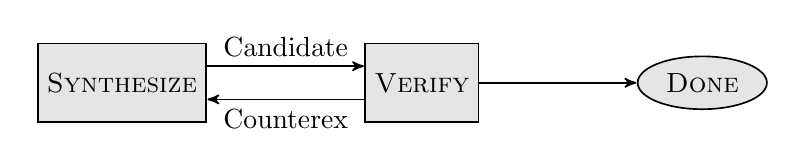
\begin{tikzpicture}[scale=0.3,->,>=stealth',shorten >=.2pt,auto,
 semithick, initial text=, ampersand replacement=\&,]

  \matrix[nodes={draw, fill=none, shape=rectangle, minimum height=.2cm, minimum width=.2cm, align=center
},
          row sep=1cm, column sep=2cm] {
   \node[fill=gray!20,minimum height=1cm] (synth) {{\sc Synthesize}};
   \&
   \node[fill=gray!20,minimum height=1cm] (verif) {{\sc Verify}};
   \&
   \node[ellipse,fill=gray!20] (done) {{\sc Done}}; 
    \\
  };

   \path
   ([yshift=2em]synth.east) edge node[align=center] {Candidate} ([yshift=2em]verif.west)
    ([yshift=-2em]verif.west) edge node[align=center] {Counterex} ([yshift=-2em]synth.east)
    (verif) edge node {} (done);
 \end{tikzpicture}
}
 \caption{The CEGIS framework\label{fig:CEGIS}}
\end{figure}

In this section, we give a brief description of the CEGIS framework~\cite{jha-icse10,
  DBLP:conf/asplos/Solar-LezamaTBSS06}, which is illustrated in Figure~\ref{fig:CEGIS}. 
  CEGIS has been recently used for the automated synthesis of software programs, 
  and its setup is naturally that of mathematical logic. 

We consider an input specification of the form 
$$
\exists P .\, \forall a.\, \phi(a, P),
$$  
where $P$ ranges over functions (where a function is represented by the program computing it),
$a$ ranges over ground terms, 
and $\phi$ is a quantifier-free logical formula. 
We~interpret the ground terms over some domain~$\mathcal{D}$. 
This is a synthesis problem, where the objective is indeed to select a valid $P$ satisfying $\phi$ over all the $a$ terms. 

CEGIS breaks down this generally hard synthesis problem into two easier parts:
%The design consists of two phases,
an inductive synthesis phase (denoted by {\sc Synthesize} in
Figure~\ref{fig:CEGIS}) and a validation phase (denoted by {\sc
  Verify}), which interact via a finite set of tests {\sc
  inputs} that is updated incrementally.
Given the specification $\phi$, the inductive synthesis procedure tries to
find an existential witness $P$ satisfying the specification
$\phi(a, P)$ for all $a$ in {\sc inputs} (as opposed to all $a \in
\mathcal{D}$).
%
If the synthesis phase succeeds in finding a witness~$P$, this witness is a
candidate solution to the full synthesis formula.  We pass this candidate
solution to the validation phase, which checks whether it is a full solution
(i.e., $P$ satisfies the specification $\phi(a, P)$ for all
$a\in\mathcal{D}$).  If this is the case, then the algorithm terminates. 
Otherwise, additional information is provided to the inductive synthesis
phase in the form of a new counterexample that is added to the {\sc inputs}
set and the loop iterates again.  %% More details about the general
%% architecture of the synthesizer can be found
%% in~\cite{DBLP:conf/lpar/DavidKL15}.
If the solution space is finite then the CEGIS loop is guaranteed to
terminate by either finding a solution or showing that no solution
exists.

In the context of the formal synthesis of safe controllers, 
the set of possible {\sc inputs} corresponds to the set of possible initial states and the 
candidate program $P$ is a candidate controllers $K$. The synthesis block generates a candidate
controller that works for a subset of the possible initial states, and the verifier checks whether 
the controller works for all possible initial states. 

%-------------------------------
\section{Formal specification of properties on a model} 
\label{sec:specification}
%-------------------------------

%While in the previous section we have discussed the generic CEGIS framework, 
In the rest of the paper we explain how to adapt the generic CEGIS framework to the synthesis of digital controllers. 
We start by describing the specific property that we pass to the synthesizer as the specification $\phi$. 
Namely, we are interested in capturing safety, 
which we discuss in Section~\ref{ssec:safespecification}. We use a stability specification 
in order to narrow the search space of possible controllers, as discussed in Section~\ref{ssec:stabspecification}.

%-------------------------------
\subsection{Formal specification of stability} 
\label{ssec:stabspecification}
%-------------------------------

There are a number of procedures that can be used for stability analysis of dynamical models~\cite{daes20161, Bessa16}, 
which can fit our automatic verification engine.  
%one based on Schur's decomposition
%and another one based on Jury's criterion~\cite{astrom1997computer}.  
Here we choose Jury stability criterion~\cite{astrom1997computer}, 
in view of its efficiency and ease of integration within our implementation.  
This method checks the stability working in the complex domain of the characteristic polynomial $S(z)$,  
%
% of the matrix $\left( \begin{array}{c} Y \\ U \end{array}\right)$, where $Y(z)$ is the closed-loop system output and U(z) is the controller output. 
%% \red{[unclear: what matrix? We need to clarify the relationship
%% between the char. poly. $S(z)$ and the later quantities $\Delta
%% N_{G}(z), \Delta D_{G}(z)$ and corresponding controller's
%% structure.]}.
%
considered in its general form as 
% for $S(z)$:
%
\begin{equation*}
S(z) = a_0z^N+a_1z^{N-1}+\cdots+a_{N-1}z+a_N,\,\, a_0\neq0. 
\end{equation*}
An LTI system is stable if all the roots of its characteristic polynomial $S(z)$ (i.e., the 
eigen values of the closed loop matrix $A_d-B_dK$) are inside the unit circle of the complex plane, 
i.e., their absolute values are less than one. 

%\note{The characteristic polynomial $S(z)$ represents the dynamical model in \ldots [clarify whether we use the CPol to describe the open- or closed-loop model. Relate parameters to matrices A,B,K. Notice that these parameters are used later in the Section where AA-based backend is explained.]}

The following matrix $M$ with dimension $(2N-2)\times N$ and elements $m_{(\cdot),(\cdot)}$ is built from the coefficients of $S(z)$ as:  
%
$$
M=\left( 
\begin{array}{c}
V^{(0)}\\
V^{(1)}\\
\vdots\\
V^{(N-2)}
\end{array}
\right), 
$$
%
where $V^{(k)} = [v^{(k)}_{ij} ]_{2\times N}$ is such that:
%
$$
v_{ij}^{(0)}=\left\{
\begin{array}{ll}
a_{j-1}, & \mbox{if}~i=1\\
v_{(1)(N-j+1)}^{0},&\mbox{if}~i=2
\end{array}
\right.
$$
%
$$
v_{ij}^{(k)}=\left\{
\begin{array}{ll}
0,&\mbox{if}~j>n-k\\
v_{1j}^{(k-1)}-v_{2j}^{(k-1)} . \frac{v_{11}^{(k-1)}}{v_{21}^{(k-1)}}, & \mbox{if}~j\leq n-k ~\mbox{and}~i=1\\
v_{(1)(N-j+1)}^{k},& \mbox{if}~j\leq n-k ~\mbox{and}~i=2\\
\end{array}
\right.
$$
%
and where $k \in \mathbb{Z}$ is such that $0 < k < N - 2$.  

We have that $S(z)$ is the characteristic polynomial of a stable system if and only if the following four conditions $R_i, i = 1,2,3,4,$ hold~\cite{astrom1997computer}:
%\begin{itemize}
%\item 
$R_1: S(1) > 0$;
%\item 
$R_2: (-1)^N S(-1) > 0$;
%\item 
$R_3: |a_0| < a_N$;
%\item 
$R_4: m_{11} > 0 \wedge\allowbreak
      m_{31}>0 \wedge\allowbreak
      m_{51}>0 \wedge \ldots \wedge\allowbreak
      m_{(2N{-}3)(1)}>0$.
%\end{itemize}

The stability property is finally encoded by a constraint expressed as the following formula: 
$
\phi_\mathit{stability} := (R_1 \wedge R_2 \wedge R_3 \wedge R_4).
$


%-------------------------------
\subsection{Formal specification of safety} 
\label{ssec:safespecification}
%-------------------------------

%We are not limited to the synthesis of digital stabilizing controllers -- a
%well known task in the literature on digital control systems -- but target
%safety requirements with an overall approach that is sound and automated. 
%More specifically, we require that the closed-loop system meets given safety specifications.  
We target synthesis of safe digital controllers with an overall approach that is sound and automated.
A safety specification translates into a requirement on the states of the closed-loop model, 
which hinges on the choice of the feedback controller (namely the choice of the gains in the matrix~$K$):  
we must ensure that the states of the closed-loop model never violate this requirement, expressed as a given subset of the state space.  

Note that a stable closed-loop model is not necessarily a safe model: 
indeed, the state values may leave the safe part of the state space while they converge
to the equilibrium, which is typical in the case of oscillatory and convergent dynamics. 
%However, a safe system will always be stable.  
In~this work, the safety property is expressed as the formula:
%
\begin{equation}
\label{eq:safetyliteral}
\phi_\mathit{safety} := \forall k\ge 0,\, \bigwedge_{i=1}^{n}{\underline{x_{i}} \leq x_{i,k} \leq \overline{x_{i}}},
\end{equation}
%
%\addtodo{We consider $x_{i}^{-}$ and $x_{i}^{+}$ to be -1 and 1, respectively.}
%
where $\underline{x_{i}}$ and $\overline{x_{i}}$ are lower and upper bounds
for the $i$-th coordinate $x_{i}$ of state $x\in \mathbb R^n$, ranging over the $k$-th time step.  
This means that the states are required to remain within an $n$-dimensional hyper-box at any point in time.  	

Furthermore, it is practically relevant to consider constraints $\phi_\mathit{input}$ on the input
signal $u_{k}$ and requirements $\phi_\mathit{init}$ on the initial states $x_0$, 
both of which we be expressed via given bounds as: 
$\phi_\mathit{input} := {\forall k\ge 0, \underline{u} \leq u_{k} \leq \overline{u}} $, 
and $\phi_\mathit{init} := \bigwedge_{i=1}^{n} \underline{x_{i,0}} \leq x_{i,0} \leq \overline{x_{i,0}}$. 
For the input signal, these requirements practically mean that the control input saturates in view of physical constraints. 

%-------------------------------
\ifx\axelerator
\subsection{Abstract acceleration of linear dynamics \note{Shall we move the material on AAccel to the Preliminaries?}} 
\label{ssec:aa}
%-------------------------------
 
We recall a technique called \emph{Abstract Acceleration}~\cite{JSS14,cattaruzza2015unbounded}, 
which will be key in this work for abstraction-based synthesis.  
Abstract Acceleration allows one to perform reachability analysis of dynamical models, 
and as such can be employed for safety verification. 
% 
Given an autonomous model of an iterative program with dynamics 
%
$\vec{x}_{k+1}=\mat{A_d}\vec{x}_k$, 
where $\vec{x}_k \in \mathbb{R}^p$, $\mat{A_d} \in \mathbb{R}^{p \times p}$ and $k \in \mathbb N_0$, 
%\end{equation}
%
we want to find all possible states visited over an infinite time horizon starting at a given initial set $X_0$.  
This set is known as the \emph{reach tube} of the model: 
%
\begin{equation}
\hat{X} = \{ \vec{x}_k: k \in \mathbb N_0, \vec{x}_0 \in X_0 \text{ and } \vec{x}_{k+1}=\mat{A_d}\vec{x}_k\}.
\end{equation}
%
Using Abstract Acceleration we transform this sequential reachability problem into a one-step problem. 
This has a lot of benefits ~\cite{JSS14}, not least in terms of numerical error propagation.   
In order to attain this, 
the problem statement is modified 
%, by means of acceleration, 
into 
%
\begin{equation}
\hat{X} = \{ \vec{x}_k=\mat{A_d}^k\vec{x}_0: k \in N_0 \text{ and } \vec{x}_0 \in X_0 \}, 
\end{equation}
%
and a new 
%model semantics and corresponding 
set $\hat{X}^\sharp$ is further defined as 
%
\begin{equation}\label{eq:aa_reachtube}
\hat{X} \subseteq \hat{X}^\sharp = \mathcal{A}X_0, \text{ such that } \bigcup_{k \in [0\ \infty)} \mat{A_d}^k \subseteq \mathcal{A}, 
\end{equation}
%
where the newly introduced \emph{abstract reach tube} $\hat{X}^\sharp$ is an
over-approximation of the reach tube of the model: 
\cite{JSS14} details algorithms to compute such set, 
whereas \cite{cattaruzza2015unbounded} extends this to LTI models with inputs as in Eqn. \eqref{eq:plant}.  
In view of the overall goal of this work, 
we extend the algorithm to continuous-time models.  
% and  For this reason we must first look at the acceleration of continuous-time dynamics.


The time discretization in Sec.~\ref{sec:model} only allows us to evaluate
the state of the plant at integer multiples of the sample time.  
%\note{Unlike the CAV18 paper, these gain matrices have not been discussed yet. }
However, in order to synthesize a soundly safe controller, 
% $\mat{K}$, 
we must be able to ensure that the safety of the plant holds at any continuous point in time.  
In order to do so, we accelerate the dynamics of the plant according to the continuous-time model
semantics in Sec.~\ref{sec:model}. 

%+++++++++++++++++++++++++++++++++++++++++++++++++++++++++++++++++++++++++++++++
\subsubsection{Accelerated\! dynamics\! for\! continuous-time\! models\! with\! parametric\! inputs}\label{sec:real_discrete_param_inputs}
%+++++++++++++++++++++++++++++++++++++++++++++++++++++++++++++++++++++++++++++++
% 
Given a specific time $T$, the state $\vec{x}(t=T)$ can be expressed as a
linear function of initial state $\vec{x}_0$ and parametric input $\vec{u}$ as follows.   
 
\begin{lemma}
The solution to the differential equation $\dot{\vec{x}}(t)=\mat{A}\vec{x}(t)+\mat{B}\vec{u}(t)$, where
$\forall t\geq 0\,\vec{u}(t)=\vec{u}$, $\mat{A}=\mat{S}\mat{J}\mat{S}^{-1}$, and $\mat{S}$ are the generalized eigenvectors of $\mat{A}$,
evaluated at time $T$ is
%
\begin{align}
\label{eq:continuous_tube_param}
\vec{x}_T&=\vec{x}(t=T)=\mat{A}_T\vec{x}_0 + \mat{B}_T\vec{u}\\
 \mat{A}_{T}&= \mat{S}
 \left [ \begin{array}{cccc}
 e^{T\lambda_1}  & s_1\frac{T^{1}e^{T\lambda_i}}{(2)!} & \hdots  & s_i\frac{T^{p-1}e^{T\lambda_i}}{(p-i)!} \\
0 & e^{T\lambda_i}  & s_i\frac{T^{j-i}e^{T\lambda_i}}{(j-i)!} & \vdots \\
\vdots & & \ddots & \vdots \\
0 & \cdots & 0  &e^{T\lambda_i} \\
\end{array} \right ]
 \mat{S}^{-1}
 \label{eq:continuous_tube_dyn2}\\
 \mat{B}_T&=\mat{A}^{-1}(\mat{I}-\mat{A}_T)\mat{B}
 \footnote{When $\mat{A}$ is not invertible,
we use $\left[\begin{array}{cc}\mat{A}_T&\mat{B}_T\\
0&\mat{I}\end{array}\right]=e^{\left[\begin{array}{cc}\mat{A}&\mat{B}\\0&0\end{array}\right]}$.}\\
 &\text{where } s_i=\left\{\begin{array}{cc}1&\quad gm(\lambda_i)>1\\0&\quad gm(\lambda_i)=1\end{array}\right.,\nonumber
\end{align}
%
$\lambda_i$ are the eigenvalues of $\mat{A}$, and $gm(\lambda_i)$ is the geometric multiplicity of $\lambda_i$.
%

If $\mat{J}$ is diagonal and there exists a sampling time $T_s$ such that $A_d=e^{\mat{A} T_s}$, 
then $\forall T \in \mathbb{R}_0^+$ we obtain the known expression 
$$
\vec{x}_T=A_d^{\frac{T}{T_s}}\vec{x}_0+(\mat{I}-\mat{A}_d^{\frac{T}{T_s}})\mat{B}_d\vec{u}, 
$$
where $\mat{A}_d^{\frac{T}{T_s}} =e^{log(\mat{A}_d) \frac{T}{T_s}} = e^{\mat{A} T}$. 
%is the state of the system at time $t=T$. 
\end{lemma}

%+++++++++++++++++++++++++++++++++++++++++++++++++++++++++++++++++++++++++++++++
\subsubsection{Accelerated dynamics for models with a sampled-time feedback}\label{sec:real_discrete_feedback_inputs}
%+++++++++++++++++++++++++++++++++++++++++++++++++++++++++++++++++++++++++++++++

We analyze the case of hybrid-time models, 
namely where the plant dynamics evolve in continuous time, 
while the feedback dynamics evolve in discrete time.  
A new input value is accepted by the plant only at sample times $T_s$.
%but implemented over the continuous-time plant dynamics.
%
%\note{Matrix K has not been introduced yet. }
\begin{theorem}
The expression
%
 \begin{align}
 \vec{x}_{T} &= (\mat{A}_{T-kT_s}-\mat{B}_{T-kT_s}\mat{K}) (\mat{A}_d-\mat{B}_d\mat{K})^k\vec{x}_0, 
 \label{eq:cyber_feedback}
 \end{align}
%
with $\mat{A}_T$ as in \eqref{eq:continuous_tube_dyn2}, $\mat{B}_T$ as in
\eqref{eq:continuous_tube_param}, and where $\mat{A}_d=\mat{A}_{T_s}$,
$\mat{B}_d=\mat{B}_{T_s}$ describe the discretized plant dynamics with
sample time $T_s$, is the state of the model
%
\begin{align*}
 \dot{\vec{x}}(t) = \mat{A}\vec{x}(t)+\mat{B}\vec{u}(t), \quad 
 \vec{u}(t)=\mat{K}\vec{x}_k,  \,
 kT_s \leq t < (k+1)T_s \,. 
\end{align*}
%
\end{theorem}
\begin{proof}
\note{let us not number the proofs.}
%
Let $\mat{K}$ be a feedback controller such that
$\vec{u}_k=-\mat{K}\vec{x}_k$ at time $t=kT_s$.  Let the output of the
feedback system be a zero order holder such that
$\vec{u}(t'+kT_s)=\vec{u}(kT_s), \text{ for } 0 \leq t' < T_s$.  The closed
loop dynamics of the system between times $kT_s$ and $kT_s+T_s$ are
%
\begin{align*}
\vec{x}_{k,t'}=\mat{A}_{t'}\vec{x}_k-\mat{B}_{t'}\mat{K}\vec{x}_k = (\mat{A}_{t'}-\mat{B}_{t'}\mat{K})\vec{x}_k,
\end{align*}
where $0 \leq t' < T_s$
We further explore the dynamics across discrete time boundaries. Let $\mat{A}_d=\mat{A}_{T_s}$ and $\mat{B}_d=\mat{B}_{T_s}$
\begin{align*}
\vec{x}_{k}&=\vec{x}_{k-1,T_s}= (\mat{A}_d-\mat{B}_d\mat{K})\vec{x}_{k-1}\\
\vec{x}_{k,T_s} &= (\mat{A}_d-\mat{B}_d\mat{K}) (\mat{A}_d-\mat{B}_d\mat{K})\vec{x}_{k-1}
\end{align*}
which accelerating results and setting $T=kT_s+t'$ becomes
\begin{align}
\label{eq:feedback_sampled_cont}
\vec{x}_{k} &= (\mat{A}_d-\mat{B}_d\mat{K}) ^k\vec{x}_0\\
\vec{x}_{T} &= (\mat{A}_{T-kT_s}-\mat{B}_{T-kT_s}\mat{K}) (\mat{A}_d-\mat{B}_d\mat{K})^k\vec{x}_0
\label{eq:feedback_cont}
\end{align}
\end{proof}

%-------------------------------
 \subsubsection{Abstract supports for continuous-time models}
 \label{sec:cont_aasup}
%-------------------------------

Just as the accelerated dynamics in Eqn. \eqref{eq:feedback_sampled_cont} can be abstracted using \eqref{eq:aa_reachtube} (where $\bigcup_{k \in N_0} (\mat{A}_d-\mat{B}_d\mat{K}) ^k \subseteq \mathcal{A}$), 
we use the same principle on Eqn. \eqref{eq:feedback_cont} to obtain 
\begin{equation}\label{eq:aa_cont_amatrix}
\bigcup_{T \in [0, T_s], k \in N_0} (\mat{A}_{T-kT_s}-\mat{B}_{T-kT_s}\mat{K}) (\mat{A}_d-\mat{B}_d\mat{K})^k \subseteq \mathcal{A}.
\end{equation}

We next describe how to obtain an over-approximation of such a set. 
This is defined as a polyhedron, expressed as an intersection of hyperplanes. 
A tight polyhedron can be obtained with hyperplanes that are tangent to the set,  
which is achieved by selecting a number of points on the boundary of the set, 
and finding corresponding hyperplanes that are tangent to those points with respect to the dynamics.  
\note{[you are essentially taking the Lie derivative of the set wrt the dynamics at the selected point?]}
In order to simplify this procedure, we look at two-dimensional cuts \note{projection?} of the space, one at a time (i.e., for every pair
of eigenvalues of the closed-loop dynamics, we find a hyperplane tangent to
the progression of that pair in a two dimensional space and use it as a face of
the polyhedron).  The difference with~\cite{cattaruzza2015unbounded} is that
in the continuous case, the tangent is found by derivation \note{cf. `Lie derivative' above} rather than
differentialtion, thus including all intermediate points \note{[?] in the arc}. 

\note{So the case study section should emphasise that the AA-based back-end can handle continuous-time benchmarks/models? 
It seems like the discussion in this section is not reflected on the case study section yet. } 

\fi
%-------------------------------
\section{Synthesis of digital controllers with CEGIS} 
\label{sssec:cegisdig}
%-------------------------------

In this section we discuss 
\ifx\axelerator
two instantiations of CEGIS: 
the first one,
named {\it multi-stage} approach, 
relies on an unfolding of the dynamics up to a completeness threshold; 
the second one is {\it abstraction-based}, 
and it leverages abstraction-refinement \cite{DBLP:conf/cav/ClarkeGJLV00} and abstract acceleration (cf. Sec.~\ref{ssec:aa}) to improve scalability,  
while retaining soundness. 
\else
the instantiation of CEGIS we use to synthesise safe digital controllers. We use a multi-stage approach
that unwinds the dynamics yup to a completeness threshold, verifying soundness using bit-precise bounded model checking.
\fi

\ifx\axelerator
%-------------------------------
\subsection{Multi-stage CEGIS} 
\label{sssec:naive}
%-------------------------------
\fi

\begin{figure*}[htb]
\scriptsize\centering
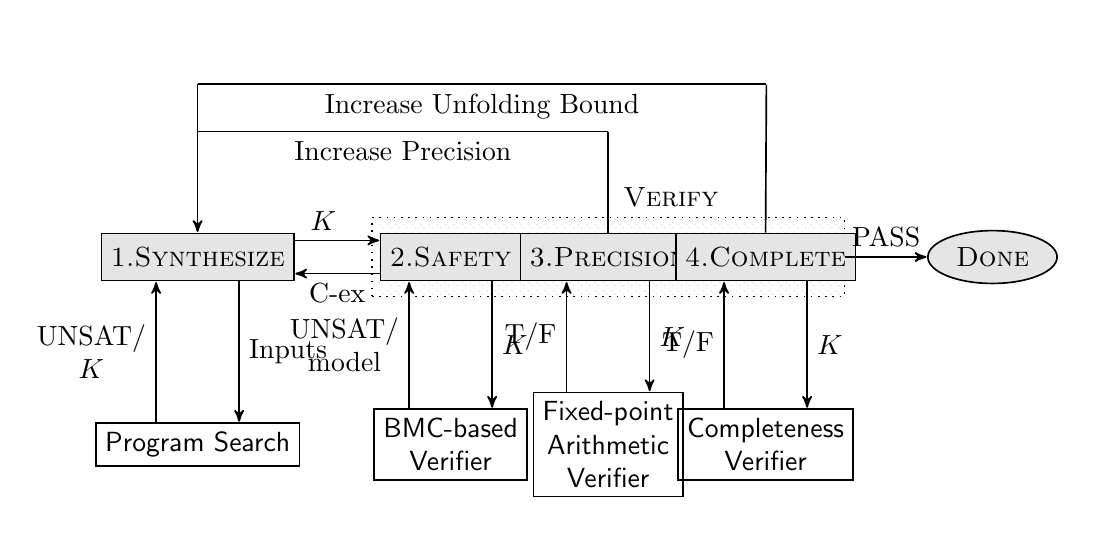
\begin{tikzpicture}[scale=0.3,->,>=stealth',shorten >=.2pt,auto, semithick, initial text=, ampersand replacement=\&,]
  \matrix[nodes={draw, fill=none, shape=rectangle, minimum height=.2cm, minimum width=.2cm, align=center},
          row sep=.6cm, column sep=.9cm] {
   \coordinate (aux1);
   \& \coordinate (aux2);
   \&;\\
   \coordinate (aux3);
   \& \coordinate (aux4);
   \&;\\
   \coordinate (aux5);
   \& \coordinate (aux6);
   \&;\\
   \node[minimum width=1.5cm, minimum height=0.6cm, fill=gray!20] (synth) {{\sc 1.Synthesize}};
   \&
   complexnode/.pic={ 
     \node[rectangle,draw,dotted,
	minimum width=6cm,
	minimum height=1cm,
        pattern=north west lines, pattern color=gray!20,
	label={\sc ~~~~~~~~~~~~Verify},] (verif) {};
     \node[minimum width=1cm, minimum height=0.6cm, fill=gray!20] (verif1) at ([xshift=-2cm]verif.center) {{\sc 2.Safety}};
     \node[minimum width=1cm, minimum height=0.6cm, fill=gray!20] (verif2) at ([xshift=0cm]verif.center) {{\sc 3.Precision}};
     \node[minimum width=1cm, minimum height=0.6cm, fill=gray!20] (verif3) at ([xshift=2cm]verif.center) {{\sc 4.Complete}};
     %\node[minimum width=1cm, minimum height=0.6cm, fill=gray!20] (verif4) at ([xshift=3.1cm]verif.center) {{\sc 5.Sampling}};
   } 
   \& \node[ellipse, fill=gray!20] (done) {{\sc Done}};\\
   \& \\
   \node[minimum height=0cm] (gp) {\sf Program Search};
   \&
   complexnode/.pic={ 
     \coordinate (aux);
   \node (bmc) at ([xshift=-2cm]aux.center) {\sf BMC-based \\ \sf Verifier};
   \node (fp)  at ([xshift=0cm]aux.center) {\sf Fixed-point \\ \sf Arithmetic\\ \sf Verifier};
   \node (sv)  at ([xshift=2cm]aux.center) {\sf Completeness\\ \sf Verifier};
   %\node (cv)  at ([xshift=3.1cm]aux.center) {\sf Sampling\\Verifier};
   }   
    \\
  };

   \path
    ([yshift=2em]synth.east) edge node[xshift=-0.5em,align=center] {$K$} ([yshift=2em]verif1.west)
    ([yshift=-2em]verif1.west) edge node {C-ex} ([yshift=-2em]synth.east)
    ([xshift=-5em]fp.north) edge node[align=center]  {T/F} ([xshift=-5em]verif2.south)
    ([xshift=-5em]sv.north) edge node[align=center]  {T/F} ([xshift=-5em]verif3.south)
    %([xshift=-5em]cv.north) edge node[align=center]  {T/F} ([xshift=-5em]verif4.south)
    ([xshift=5em]verif1.south) edge node[align=center] {$K$} ([xshift=5em]bmc.north)
    ([xshift=5em]verif2.south) edge node[align=center] {$K$} ([xshift=5em]fp.north)
    ([xshift=5em]verif3.south) edge node[align=center] {$K$} ([xshift=5em]sv.north)
    %([xshift=5em]verif4.south) edge node[align=center] {$K$} ([xshift=5em]cv.north)
    ([xshift=-5em]bmc.north) edge node[align=center]  {UNSAT/\\model} ([xshift=-5em]verif1.south)
    (verif) edge node {PASS} (done)
    ([xshift=5em]synth.south) edge node[align=center] {Inputs} ([xshift=5em]gp.north)
    ([xshift=-5em]gp.north) edge node[align=center] {UNSAT/\\$K$} ([xshift=-5em]synth.south)
    (aux3) edge (synth.north);
   \path[-]
   (verif2.north) edge node[align=center] {} ([xshift=0cm]aux6)
   ([xshift=0cm]aux6) edge node[align=center] {Increase Precision} (aux5)
   (verif3.north) edge node[align=center] {} ([xshift=6.7cm]aux4)
   ([xshift=6.7cm]aux4) edge node[align=center] {Increase Unfolding Bound} (aux3);
   %(verif4.north) edge node[align=center] {} ([xshift=10.5cm]aux2)
   %([xshift=10.5cm]aux2) edge node[align=center] {Increase Sampling Rate} (aux1);
\end{tikzpicture}
\caption{CEGIS with multi-staged verification}
\label{fig:CEGIS-precision-increment}
\end{figure*}

%\subsubsection{Controller synthesis}

An overview of the algorithm for controller synthesis is given in Figure~\ref{fig:CEGIS-precision-increment}.   
One important point is that we formally synthesize a controller over a finite number ($k$) of time steps.  
We then compute a completeness threshold $\overline{k}$~\cite{DBLP:conf/vmcai/KroeningS03} for this controller, 
and verify the correct behaviour for $\overline{k}$ time steps. 
As we will later argue, $\overline{k}$ is the number of iterations required to sufficiently unwind the dynamics of the closed-loop state-space model,  
ensuring that the safety boundaries are not violated for any other $k{>}\overline{k}$. 

%\begin{theorem} There exists a finite $\overline{k}$ such that it is
%sufficient to unwind the closed-loop state-space system up to $\overline{k}$
%in order to ensure that $\phi_\mathit{safety}$ holds. 
%\end{theorem}
%
%\begin{proof}
%%
%A stable control system is known to have converging dynamics.  Assume the
%closed-loop matrix eigenvalues are not repeated (which is sensible to do,
%since we select them).  The distance of the trajectory from the reference
%point (origin) decreases over time within subspaces related to real-valued
%eigenvalues; however, this is not the case in general when dealing with
%complex eigenvalues.  Consider the closed-loop matrix that updates the
%states in every discrete time step, and select the eigenvalue $\vartheta$
%with the smallest (non-trivial) imaginary value.  Between every pair of
%consecutive time steps $k\,T_s$ and $(k+1)\,T_s$, the dynamics projected on
%the corresponding eigenspace rotate $\vartheta T_s$ radians.  Thus, taking
%$\overline{k}$ as the ceiling of $\frac{2\pi}{\vartheta T_s}$, after
%$k{\geq}\overline{k}$ steps we have completed a full rotation, which results
%in a point closer to the origin.  The synthesized $\overline{k}$ is the completeness threshold.
%\qed 
%%
%\end{proof}
%
%\medskip

Next, 
with reference to the CEGIS scheme in Figure~\ref{fig:CEGIS}, 
we describe in detail the different phases in Fig.~\ref{fig:CEGIS-precision-increment} (shaded blocks 1 to 4). 

%\note{we need to refer to the parts of Algorithm 1 more closely - point to specific lines in the explanation below.} 

%\todo{please eventually itemize next}
\begin{enumerate}

\item The inductive synthesis phase ({\sc synthesize}) uses BMC to compute a
candidate solution $K$ that satisfies both the stability criteria and the
safety specification.  

To synthesize a controller that satisfies the 
stability criteria, we require that a computed polynomial satisfies Jury's
criterion~\cite{fadali} (see Section~\ref{ssec:stabspecification}).

Regarding the second requirement, 
we fix an index $k$, 
and we synthesize a safe controller by
unfolding the transition system $k$ steps and by selecting a controller $K$ and a single initial state, 
such that the states at each step do not violate the safety criteria (see Section~\ref{ssec:safespecification}).    
That is, we ask the bounded model checker~\cite{ClarkeKL04} if there exists a $K$ that is safe for at least one $x_0$ in our set of all possible initial states, and a given fixed point precision for the controller, and where the input signal remains within the specified bounds.
This approach is sound if the current $k$ is greater than the completeness threshold (see later step).  
We~also assume some (fixed or floating point) precision $\langle I_p,F_p\rangle$ for the plant and a sampling rate.  
The checks that these assumptions hold are performed by subsequent {\sc verify} stages. 


%\begin{algorithm}[]
%\scriptsize
%\begin{algorithmic}[1]
%\Function{$stabilityCheck()$}{}
%  \State computecharPoly($A_d - B_dK$)
%  \State assert(Jury's criteria hold)
  %\State Return $K$
%\EndFunction
%\end{algorithmic}
%\label{alg:stabilitycheck}
%\end{algorithm}


\begin{algorithm}[]
%\scriptsize
\begin{algorithmic}[1]
\Function{$\mathit{safetyCheck}()$}{}
\State assert($ \underline{u}  \leq u \leq \overline{u}$)
 \State set $x_0$ to be a vertex state, e.g., $[\underline{x_0},\underline{x_0}]$	
\For {($c=0;~c < 2^\mathit{Num\_States};~c\mbox{++}$) }
  %\State assert($ \underline{x_0}  \leq x_0 \leq \overline{x_0}$)
	\For{($i=0;~i< k;~i\mbox{++}$)}
		%\State $u = (\langle I_p,F_p\rangle)((\langle I_c,F_c\rangle)K * (\langle I_c,F_c\rangle) x)$
		\State $u = (plant\_typet)((controller\_typet)K * (controller\_typet) x)$
		\State $x = A * x + B * u$
		\State assert($\underline{x} \leq x \leq \overline{x}$ )
  	\EndFor
  	\State set $x_0$ to be a new vertex state
  	\EndFor
  %\State Return $K$
\EndFunction
\end{algorithmic}
\caption{Safety check\label{alg:safetycheck}}
\end{algorithm}

\item The first {\sc verify} stage, {\sc safety} is shown in Alg.~\ref{alg:safetycheck}. 
The algorithm checks that the candidate
solution $K$, which we synthesized to be safe for at least one initial
state, is safe for \emph{all} possible initial states, i.e., does not reach
an unsafe state within $k$ steps.  After unfolding the transition system corresponding
to the previously synthesized controller $k$ steps, we check that the safety
specification holds for any initial state. 

We use $(controller\_typet)$ to denote a
cast or conversion to the controller precision, and $(plant\_typet)$ to denote a cast or conversion to the 
plant precision. A \emph{vertex state} is defined as a state where all values are either equal to the upper or lower
bound of the initial states. It is sufficient to verify that the controller is safe for all vertex
states, and the proof is shown later in this section. We thus only need to iterate through the $2^{Num\_States}$ vertex
states, where $Num\_States$ is the number of dimensions in $x$.


\begin{theorem} 
If a controller is safe for each of the corner cases of our hypercube of
allowed initial states, i.e., the vertex states, it is safe for any initial state in the hypercube. 
\end{theorem}

Thus we only need to check $2^n$ initial states, where $n$
is the dimension of the state space (number of continuous variables). 
\begin{proof}
Consider the set of initial states, $X_0$, which we assume to be convex since it is a hypercube. 
Name $v_i$ its vertexes, where $i=1,\ldots, 2^n$.  
Thus any point $x \in X_0$ can be expressed by convexity as $x = \sum_{i=1}^{2^n} \alpha_i v_i$, 
where $\sum_{i=1}^{2^n} \alpha_i =1$. Then if $x_0=x$, we obtain 
\begin{align*}
x_k   &= (A_d - B_d K)^k x \\
&= (A_d - B_d K)^k \sum_{i=1}^{2^n} \alpha_i v_i \\
      &= \sum_{i=1}^{2^n} \alpha_i (A_d - B_d K)^k v_i \\
      &= \sum_{i=1}^{2^n} \alpha_i x_k^i, 
 \end{align*}     
%
where $x_k^i$ denotes the trajectories obtained from the single vertex
$v_i$.  We~conclude that any $k$-step trajectory is encompassed, within a
convex set, by those generated from the vertices. 
\qed
\end{proof}



\item The second {\sc verify} stage, {\sc precision}, 
 restores soundness with respect to the plant precision
by using interval arithmetic \cite{moore1966interval} to validate the 
operations performed by the previous stage. 

\item The third {\sc verify} stage, {\sc complete}, checks that the current
$k$ is large enough to ensure safety for any $k'{>}k$.  Here, we compute the
completeness threshold $\overline{k}$ for the current candidate controller $K$ and
check that $k{\geq}\overline{k}$.  This is done by computing the number of time steps
required for the states to have completed a 360\textdegree circle, as illustrated in Fig.~\ref{fig:ct}. 

\begin{theorem} There exists a finite $\overline{k}$ such that it is
sufficient to unwind the closed-loop state-space system up to $\overline{k}$
in order to ensure that $\phi_\mathit{safety}$ holds. 
\end{theorem}

\begin{proof}
%
A stable control system is known to have converging dynamics.  Assume the
closed-loop matrix eigenvalues are not repeated (which is sensible to do,
since we select them).  The distance of the trajectory from the reference
point (origin) decreases over time within subspaces related to real-valued
eigenvalues; however, this is not the case in general when dealing with
complex eigenvalues.  Consider the closed-loop matrix that updates the
states in every discrete time step, and select the eigenvalue $\vartheta$
with the smallest (non-trivial) imaginary value.  Between every pair of
consecutive time steps $k\,T_s$ and $(k+1)\,T_s$, the dynamics projected on
the corresponding eigenspace rotate $\vartheta T_s$ radians.  Thus, taking
$\overline{k}$ as the ceiling of $\frac{2\pi}{\vartheta T_s}$, after
$k{\geq}\overline{k}$ steps we have completed a full rotation, which results
in a point closer to the origin.  The synthesized $\overline{k}$ is the completeness threshold.
\qed 
%
\end{proof}

\end{enumerate}



\begin{figure}[t]
\centering
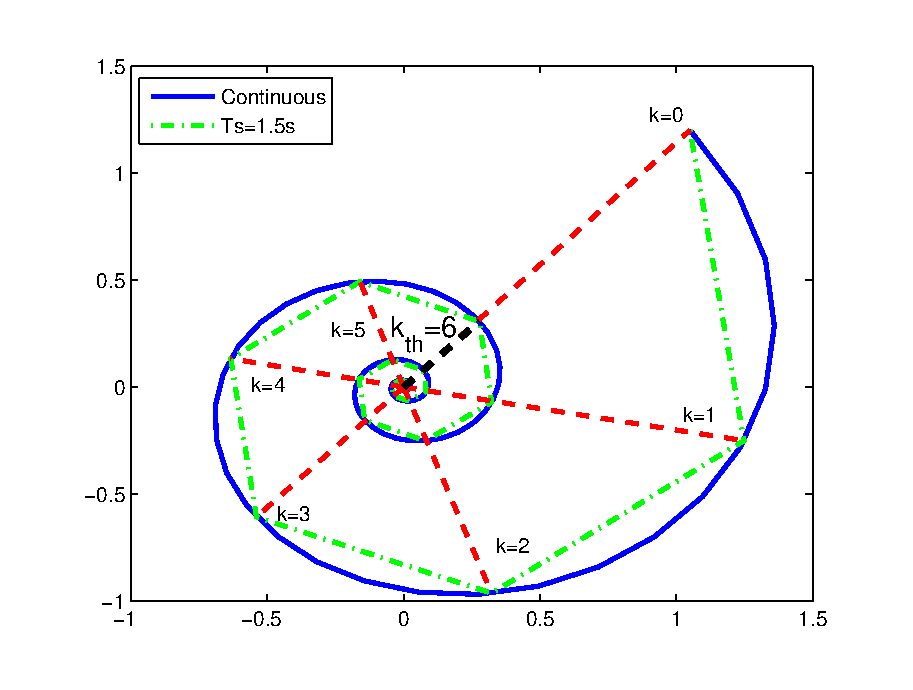
\includegraphics[width=\columnwidth]{figures/ct.eps}
%\vspace{0.1cm}
\caption{Completeness threshold for multi-staged verification. $T_s$ is the time step for the time discretization of the control matrices.}
\label{fig:ct}
\end{figure}

%Checking that the safety specification holds for any initial state can be
%computationally expensive if the bounds on the allowed initial states are
%large. \note{we have not discussed the bounds on the input signal. }

\ifx\axelerator
%-------------------------------
\subsection{Abstraction-based CEGIS} 
\label{sssec:abstraction}
%-------------------------------


The multi-staged approach above relies on the symbolic simulation over a bounded time horizon of individual initial states and inputs, 
and on the generalization to continuous sets and over an infinite time horizon. 


Conversely, in this section we synthesise a controller for continuous set of initial states and of inputs, 
over an abstraction of the continuous dynamics \cite{cattaruzza2015unbounded} that conforms to witness proofs at specific times.   
Moreover, this approach uses abstraction-refinement \cite{DBLP:conf/cav/ClarkeGJLV00},  
enabling one to start with a very simple description of the dynamics regardless of the model complexity (abstraction step), 
and only to elaborate this description 
%to more complex models 
when a solution cannot be found (refinement step). 

The CEGIS loop for this approach is illustrated in Figure~\ref{fig:CEGARIS}. 
%

It comprises the following steps:  
\begin{enumerate}
\item 
  We start by doing some preprocessing:%%  that 
  %% can be computationally intensive and we don't want it to be part of the CEGIS loop.
% Let us recall the formulas used for single-input and single-output (SISO) systems 
  % in sections \ref{sec:reachable} and \ref{sec:observable}.
  \begin{enumerate}
\item Compute the characteristic polynomial of the matrix $(A_d-B_dK)$ as 
$P_a(z) = z^n+\sum_{i=1}^n{(a_i-k_i)z^{n-i}}$.  As with the multi-staged approach, this polynomial must satisfy Jury's criterion.
\reply{The polynomial $P_a(z)$ is obtained by transforming the system into controllable form( See~\cite{astrom1997computer}, where both the dynamics and the controller are multiplied by a matrix $\mat{T}$ (derived from $\mat{A}$ and $\mat{B}$), which is given to the synthesiser.  The synthesizer is thus able to provide a $\mat{K}$ such that $k_i$ are the elements  of $\mat{K}\mat{T}^{-1}$.
}


\item Calculate the noise set $N$ from the quantizer resolutions and estimated round-off errors as follows: 

\begin{align*}
\nonumber
\begin{split}
N=\left \{ \nu_1+\nu_2+ \nu_3: \nu_1 \in \left[-\frac{q_1}{2}\ \ \frac{q_1}{2}\right] , \right. \\ \left. \nu_2 \in \left[-\frac{q_2}{2}\ \ \frac{q_2}{2}\right],  \nu_3 \in \left[-q_3\ \ q_3\right]  \right \}, 
\end{split}
\end{align*}
%
where  $q_1$ is the error introduced by the truncation in the ADC (Q1 in Fig. \ref{fig:digitalsystem}), 
$q_2$ is the error introduced by the DAC (Q2 in Fig. \ref{fig:digitalsystem}), 
and $q_3$ is the maximum truncation and rounding error in $u_k=-K \cdot \mathcal{F}_{\langle I_c,F_c \rangle}(x_k)$, 
as further discussed in Section~\ref{sec:numeric_rep}.

\item Calculate a set of initial bounds on $K$, $\phi(K)=\phi_\mathit{init}^{K}$,
based on the constraints %\blue{[how is this practically done?With the equation below]}.  
%
$$
\phi_\mathit{init}^{K} := (\phi_\mathit{init} \wedge \phi_\mathit{input} \wedge u_k=-K x_k)
$$
Note that these bounds will be used by the {\sc synthesize} phase to reduce the size of the solution space.
The specification $\phi(K)$ will later be updated by the {\sc abstract} phase to include the possible refinements. 

\end{enumerate}
\item In the {\sc synthesize} phase, we synthesize a candidate controller
  $K$ 
  that satisfies
  $\phi_\mathit{stability} \wedge \phi (K)$ by invoking a SAT solver.  
  The safety specification given to the SAT formula is an over-approximation of the original safety specification that only has constraints for a given set of iterations ($k$) and initial values.  
 The program search algorithm is as in the multi-staged approach.  
If there is no candidate solution we return UNSAT and exit the loop. 
\item Once we have a candidate solution, we perform a safety verification 
  of the 
  %consisting of evaluating the
  progression of the system from $\phi_\mathit{init}$ over time,
$x_{k} \models \phi_\mathit{safety}$. 
  In order to compute the progression of point $x_0$ at iteration $k$,
  we consider the solution of the closed-loop model 

{
\scriptsize
\begin{align*}
%\begin{split}
x=(A_d-B_dK)^kx_0+ \sum_{i=0}^{k-1} (A_d-B_dK)^i B_{n}(\nu_1+\nu_2+\nu_3), 
%\end{split}
\end{align*}
}
where $B_n= [1 \cdots 1]^T$. 
As we require to verify the closed-loop model for any $k$ up to infinity, 
we use Abstract Acceleration again to compute the reach-tube, 
i.e., the set of all reachable states at all times given an initial set
$\phi_\mathit{init}$:
%
\begin{align}
\label{eq:aa_observer_LTI_cf}
\hat{X}^\#
=\mathcal{A} X_0 + \mathcal{B}_{n} N, \,
X_0 =\left \{x: x \models \phi_\mathit{init} \right\}, 
\end{align} 
%
where $\mathcal{A}=\bigcup_{k=1}^\infty (A_d-B_dK)^k,
\mathcal{B}_{n}=\bigcup_{k=1}^\infty \sum_{i=0}^k(A_d-B_dK)^iB_{n}$ are
abstract matrices for the closed-loop system~\cite{cattaruzza2015unbounded},
whereas the set $N$ is obtained above. 

\note{What about the continuous-time abstract acceleration? Where in the case studies? }

We next evaluate whether $\hat{X}^\# \models \phi_\mathit{safety}$ using set inclusion, cf. Section \ref{sec:cont_aasup}: 
the faces of the polyhedra described by $\hat{X}^\#$ and $\phi_\mathit{safety}$ are aligned, so we only need to check that all the supports of $\hat{X}^\#$ are smaller.   
If the verification holds we have a solution, and exit the loop with a PASS.  Otherwise, we
find a counterexample iteration $k$ and corresponding initial condition $x_0$
for which the property does not hold, which we use to locally refine the
abstraction by adding the constraint $\mat{A}^k\vec{x}_0 \models \phi_\mathit{safety}$ (which is calculated explicitly using acceleration for the given $k$ and $\vec{x}_0$).  
When the abstraction cannot be further refined, we provide $(k, x_0)$ to the {\sc abstract} phase.

\item If we reach the {\sc abstract} phase, it means that the candidate solution is not valid,
  in which case we must refine the abstraction used by the synthesizer.
\begin{enumerate}
\item Find the constraints that invalidate the property ($\{ k, x_0 : \mat{A}^k\vec{x}_0 \not \models \phi_\mathit{safety}\}$) as a set of counterexamples for the eigenvalues, which we define as $\phi_\Lambda=\{ k, x_0 : \mat{J}^k\mat{S}^{-1}\vec{x}_0 \models \phi_\mathit{safety}\}$. 
This is a constraint for the spectrum of the closed-loop dynamics.  
\item We use $\phi_\Lambda$ to
  further constrain the characteristic polynomial %\blue{[again, check the coefficients of the characteristic polynomial.]I don't find any error} 
$z^n+\sum_{i=1}^n(a_i-k_i)z^{n-i}=\prod_{i=1}^n (z-\lambda_i) \text{ where } |\lambda_i|<1 \wedge \lambda_i \models \phi_{\Lambda}$. These constraints correspond to specific iterations for which the system may be unsafe.
\item Pass the refined abstraction $\phi(K)$ with the new constraints and the list of iterations $k$ to the {\sc synthesize} phase (step (2)).
  %, as well as a counterexample plant coefficients ($P_a$) and repeat the loop again. 
\end{enumerate} 
\end{enumerate}


\begin{figure*}
\centering\scriptsize
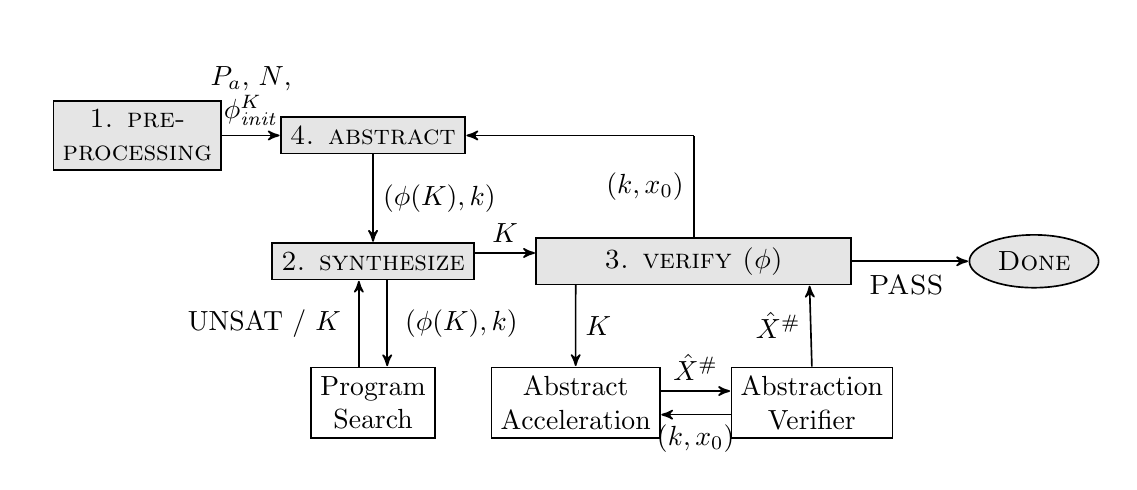
\begin{tikzpicture}[scale=0.3,->,>=stealth',shorten >=.2pt,auto, semithick, ampersand replacement=\&,]
  \matrix[nodes={draw, fill=none, shape=rectangle, minimum height=.2cm, minimum width=.2cm, align=center},row sep=.8cm, column sep=.2cm] {
   \coordinate (aux1);
   \& \coordinate (aux2);
   \& ;\\
   \&\node[fill=gray!20,align=center,xshift=-1.5cm] (pre) {{\sc 1. pre-}\\{\sc processing}};
   \& \node[fill=gray!20,align=center] (abstract) {\sc 4. abstract};
   \& \coordinate (aux); \\ 
   \&
   \& \node[fill=gray!20,align=center] (synth) {\sc 2. synthesize};
   \& \node[fill=gray!20,align=center, minimum width=4cm] (verify) {\sc 3. verify ($\phi$)};
      \node[draw=none] (SAT) at ([xshift=2.7cm,yshift=-.3cm]verify)  {\sc PASS};
   \& \node[ellipse, fill=gray!20] (done) {{\sc Done}};\\
   \&
   \& \node[draw,rectangle,align=center] (KSAT) {Program \\ Search};
   \& complexnode/.pic={
     \coordinate (AA);
     \node[draw,rectangle,align=center] (AAV) at ([xshift=-1.5cm]AA.center) {Abstract\\Acceleration};
     \node[draw,rectangle,align=center] (AAC) at ([xshift=1.5cm]AA.center) {Abstraction \\ Verifier};
    }\\
  };
  \path
    (pre.east) edge node[align=center] {$P_a$, $N$,\\ $\phi_\mathit{init}^K$} (abstract.west)
    (abstract.south) edge node{$(\phi(K), k)$} (synth.north)
    ([yshift=1em]synth.east) edge node {$K$} ([yshift=1em]verify.west)
    (aux) edge (abstract.east) 
    (verify.east) edge (done.west);
  \path
    ([xshift=-.6cm]KSAT.north) edge[left] node[xshift=-.1cm] {UNSAT / $K$} ([xshift=-0.6cm]synth.south) 
    ([xshift=.6cm]synth.south) edge node[align=center,xshift=.1cm] {$(\phi(K),k)$} ([xshift=.6cm]KSAT.north)
    ([yshift=.5cm]AAV.east) edge node{\sl $\hat{X}^\#$} ([yshift=.5cm]AAC.west)
    ([yshift=-.5cm]AAC.west) edge node{$(k,x_0)$} ([yshift=-.5cm]AAV.east)
    (AAC.north) edge node{\sl $\hat{X}^\#$} ([xshift=4.9cm]verify.south)
    ([xshift=-5cm]verify.south) edge node{$K$} (AAV.north);
  \path[-] 
     (verify.north) edge node {$(k,x_0)$} (aux);
\end{tikzpicture}
\caption{Abstraction-based CEGIS}
\label{fig:CEGARIS} 
\end{figure*} 

\fi
%+++++++++++++++++++++++++++++++++++++++++++++++++++++++++++++++++++++++++++++++
\section{Numerical representation and soundness} 
\label{sec:numeric_rep}
%+++++++++++++++++++++++++++++++++++++++++++++++++++++++++++++++++++++++++++++++

As discussed in Section~\ref{sec:errors}, 
the models we consider must account for errors from several sources: 
we must bound the numerical error introduced by the finite precision we use to represent the plant (and its operations), and precisely model
the error introduced by the ADC/DAC conversions
and the error introduced by the limited precision used to represent the controller. 
We use interval arithmetic to bound the error introduced by the finite precision plant, and bounded model checking to precisely model the error introduced by the ADC/DAC and the finite precision controller.


\subsection{Bit-precise symbolic model checking}
As described in section~\ref{sec:preliminaries}, we use CBMC, a bit-precise bounded model checker to synthesise and verify candidate controllers. CBMC performs precisely the fixed or floating point arithmetic used in the controller, as well as the ADC/DAC conversions, according to the IEEE standards.

\subsection{Interval arithmetic over errors in numeric representation} 
We use finite-precision arithmetic to model the plant. This is an approximation that speeds up each CEGIS
iteration but necessitates a further stage where we verify that the errors introduced by the
approximation have not caused us to generate a controller that is unsafe when executed with real numbers 
for the plant. In this stage, we represent the plant using double precision floating point
and we use the Boost interval arithmetic library~\cite{} to bound the error in this representation. We use a compositional numeric library to perform the fixed point arithmetic for the controller~\cite{}. We check the controller is safe starting from each vertex state, which we have shown to be sufficient to prove safety from any initial state in the hypercube of possible initial states. 

We outline here the mathematics behind bounding the errors on the double precision floating point.
Recall we use $\mathcal{F}_{\langle E,M \rangle}(x)$ denote a real number $x$
represented in a floating point domain, with $E$ bits representing the exponent and $M$ bits representing the mantissa part. Any representation of a real number using the floating point domain will
introduce an error, for which an upper bound can be given~\cite{DBLP:conf/arith/BrainTRW15}.
For each number represented in floating point, we store an interval that encompasses this error.
Further
mathematical
operations performed at the precision $\mathcal{F}_{\langle E,M \rangle}(x)$
will propagate these errors forward and 
introduce further errors for which bounds can be derived~\cite{DBLP:conf/arith/BrainTRW15}. 

The fixed point arithmetic of the digital controller is performed on the upper and lower limit of each interval independently. Since the precision of the floating point is greater than the precision
of the controller, this is guaranteed to bound the real behaviour of the controller.



\ifx\axelerator


\begin{enumerate}

\item {\bf Truncation:} Let $x$ be a real number, and $\mathcal{F}_{\langle
I,F \rangle}(x)$ be the same number represented in a fixed-point domain as
above.  Then $\mathcal{F}_{\langle I,F \rangle}(x) = x-\delta_T$ where the
error $ \delta_T=x\ \%_{c_m}\ \tilde x$ \note{define tilde x}, and $\%_{c_m}$ is the modulus
operation performed on the last bit. 
Thus, $\delta_T$ is the truncation error and it will propagate across
operations.
%
\item {\bf Rounding:} The following errors are due to basic arithmetic operations.  
Let $c_1, c_2$ and $c_3$ be real numbers, and $\delta_{T1}$ and $\delta_{T2}$ be
the truncation errors caused by representing $c_1$ and $c_2$ in a fixed-point domain.
%
\begin{enumerate}
%
\item Addition/Subtraction: these operations only propagate errors coming
from truncation of the operands, namely $\mathcal{F}_{\langle I,F
\rangle}(c_1) \pm \mathcal{F}_{\langle I,F \rangle}(c_2) = c_3 + \delta_3$
with $|\delta_3| \leq |\delta_{T1}| + |\delta_{T2}|$.
%
\item Multiplication: $\mathcal{F}_{\langle I,F \rangle}(c_1) \cdot
\mathcal{F}_{\langle I,F \rangle}(c_2) =  c_3 + \delta_3$ with $|\delta_3|
\leq |\delta_{T1}\cdot\mathcal{F}_{\langle I,F \rangle}(c_2)|\allowbreak +
|\delta_{T2}\cdot\mathcal{F}_{\langle I,F \rangle}(c_1)| + c_m$, where
$c_m=2^{-F}$ as above.
%
\item Division: the operations performed by the controllers in the FWL
domain do not include division.  However, we do use division in computations within the plant.  
Here the error depends on whether the divisor is greater or smaller than the dividend:  $\mathcal{F}_{\langle I,F
\rangle}(c_1) / \mathcal{F}_{\langle I,F \rangle}(c_2) = c_3 + \delta_{T3}$, 
where $\delta_{T3}$ is $(\delta_{T2}\cdot c_1 - \delta_{T1}\cdot
c_2)/(\delta_{T2}^2 - \delta_{T2} c_2)$,
%
%$\mathcal{F}_{\langle I,F \rangle}(c_1) / \mathcal{F}_{\langle I,F \rangle}(c_2) =  (c_1 - \delta_{T1})/ (c_2 + \delta_{T2}) + c_m $, where $c_m=2^{-F}$ as above.
\end{enumerate}

\item {\bf Overflow:}
The maximum size of a real number $x$ that can be represented in a fixed
point domain as $\mathcal{F}_{\langle I,F \rangle}(x)$ is $\pm
(2^{I-1}+1-2^{-F})$.  Numbers outside this range cannot be represented by
the domain.  If overflow occurs, the interval bound becomes infinite.

\end{enumerate}

Similar bounds for errors introduced by 
performing basic mathematical operators in floating-point precision can be derived~\cite{DBLP:conf/arith/BrainTRW15}.


\subsection{ADC/DAC quantization errors modelled as noise} 
%+++++++++++++++++++++++++++++++++++++++++++++++++++++++++++++++++++++++++++++++
In this section we describe how quantization errors can be modelled as noise. 
Note that this is only applicable to the acceleration back end, as the multi-stage back 
end makes use of CBMC's bit-precise model checking capabilities to account 
for these deterministic errors.

During any given ADC conversion, the continuous signal will be sampled in
the real domain and transformed by $\mathcal{F}_{\langle I_{c},F_{c} \rangle}
(x)$ (assuming the ADC discretization is the same as the digital
implementation).  This sampling uses a threshold which is defined by the
less significant bit ($q_{c}=c_{m_c}=2^{-F_c}$) 
%\blue{[this quantity was named $c_m$ above and in other parts of the paper - please uniformise notations]}
of the ADC and some non-linearities of the circuitry.  The overall conversion is
%
$$\mathcal{F}_{\langle I_{c},F_{c} \rangle}(x(t)) = x_k :
(x_k)_i \in \left[x_i(t)-\frac{q_{c}}{2}\ \ \ \ x_i(t)+\frac{q_{c}}{2}\right] \,.$$
%
\reply{where $x_i$ is the $i^{th}$ component of the vector $x$.}
If we denote the error in the conversion by $\nu_k=x_k-x(t)$ where $t = nk$,
and $n$ is the sampling time and $k$ the number of steps, then we may define
some bounds for it $(\nu_k)_i \in [-\frac{q_{c}}{2}\ \ \frac{q_{c}}{2}]$.

As stated before, we assume that the domain of the
ADC is that of the digital controller (i.e, the quantizer includes any
digital gain added in the code).  The process of quantization in the DAC is
similar except that it is calculating $\mathcal{F}_{\langle I_{dac},F_{dac}
\rangle} (\mathcal{F}_{\langle I_{c},F_{c} \rangle }(x)) $.  If these domains
are the same ($I_{c}=I_{dac},\allowbreak F_{c}=F_{dac}$), or if the DAC
resolution in higher than the ADC, then the DAC quantization error is equal
to zero.  From the above equations we can now define the ADC and DAC
quantization noises ${\nu_1}_k \in [-\frac{q_1}{2}\ \ \frac{q_1}{2}]$ and
${\nu_2}_k \in [-\frac{q_2}{2}\ \ \frac{q_2}{2}]$, where $q_1=q_{c}$ and 
$q_2=q_\mathit{dac}$.  This is illustrated in
Fig.~\ref{fig:digitalsystem} where $Q_1$ is the quantizer of the ADC
and $Q_2$ the quantizer for the DAC.  These bounds hold irrespective of
whether the noise is correlated, hence we may use them to over-approximate
the noise effect on the state space progression over time.  The
resulting dynamics are
%
\begin{align*}
%\label{eq:pre_quantization}
{x}_{k+1} = {A}_d{x}_k+{B}_d({u}_k+{{\nu}_2}_k), \quad u_k = -K{x}_{k}+{{\nu}_1}_k, 
\end{align*}
%
which result in the following closed-loop dynamics:
%
\begin{align*}
%\label{eq:quantization}
{x}_{k+1} &= ({A}_d-{B}_d{K}_d) {x}_k+{B}_d{{\nu}_2}_k +{{\nu}_1}_k \,. 
\end{align*}

\fi


\subsection{Effect on safety specification and stability}

Let us first consider the effect of the quantization errors on safety. 
Within the controller, state values are manipulated at low precision,
alongside the vector multiplication $Kx$.
The inputs are computed using the following equation: 
%
\begin{align*}
u_{k}&=-(\mathcal{F}_{\langle I_c,F_c \rangle}(K)\cdot\mathcal{F}_{\langle I_c,F_c \rangle}(x_{k})). 
\end{align*}

This induces two types of the errors detailed above: first, the truncation
error due to representing $x_k$ as $\mathcal{F}_{\langle I_c,F_c
\rangle}(x_{k})$; and second, the rounding error introduced by the
multiplication operation.  

An additional error is due to the representation of the plant dynamics, namely 
%
{\scriptsize
\begin{equation}
x_{k+1} =\mathcal{F}_{\langle I_p,F_p \rangle}(A_d) \mathcal{F}_{\langle I_p,F_p \rangle}(x_{k}) + \mathcal{F}_{\langle I_p,F_p \rangle}(B_d)\mathcal{F}_{\langle I_p,F_p \rangle}(u_{k}).
\end{equation}
}
We address this error by use of interval
arithmetic~\cite{moore1966interval} in the verification phase.

Previous studies~\cite{gangli1} show that the FWL affects the poles and
zeros positions, degrading the closed-loop dynamics, causing steady-state
errors and eventually de-stabilizing the system~\cite{Bessa16}.  However,
since in this paper we require stability only as a precursor to safety, it
is sufficient to check that the (perturbed, noisy) model converges to a
neighborhood of the equilibrium within the safe set.

In the following, we shall disregard these steady-state errors (caused by
FWL effects) when stability is ensured by synthesis, and then verify its
safety accounting for the finite-precision errors.



%-------------------------------
\section{DSSynth: An Automated Digital Controller Synthesis Tool for Physical Plants}
\label{sec:dssynthtool}
%-------------------------------

\begin{figure*}[t]
\centering
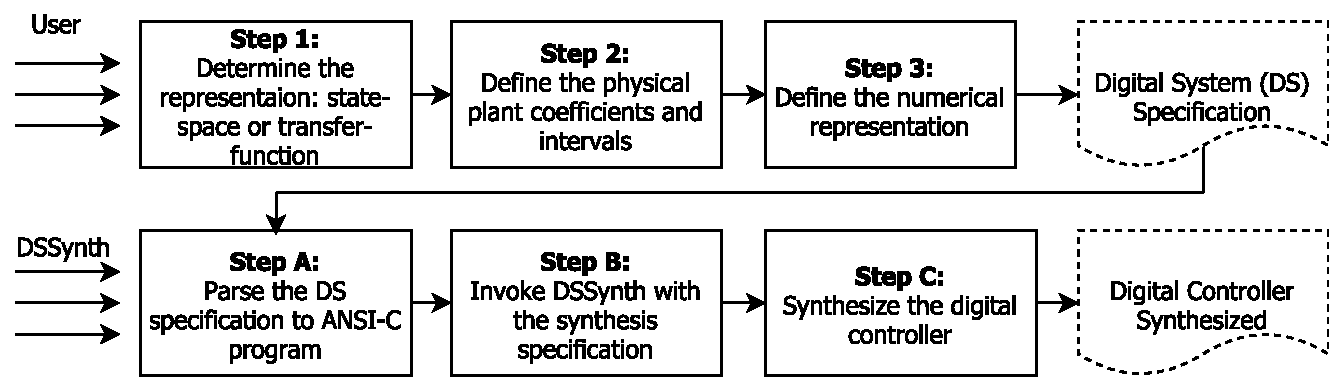
\includegraphics[width=0.7\textwidth]{figures/synthesis-flow.pdf}
\caption{Phases of the controller synthesis}
\label{fig:synthesis-flow}
\end{figure*}

The proposed synthesis methodology for closed-loop digital control
systems is based on the Digital-System Synthesizer 
(DSSynth) tool~\cite{DBLP:conf/kbse/AbateBCCCDKKP17}, 
which can be split into two main stages as follows: manual and 
automated steps, as illustrated in Fig.~\ref{fig:synthesis-flow}. 

In Step~1, the user selects the closed-loop digital control
system representation, which can be a transfer function or a state-space model.  
In Step~2, the physical plant (e.g., in the form of Equation~\eqref{eq:ode1}) must be
given~\cite{astrom1997computer}.  Finally, in Step~3, the numerical
representation for the digital controller implementation must be set by the
user, i.e., the FWL format that defines the number of bits of the integer
and fractional parts when using fixed-point arithmetic or half- and single-precision 
when using floating-point arithmetic as well as the dynamic range inputs.  The input 
provided by the user is a specification of the physical plant.

After that, the automated synthesis process starts with Step~A, where the
\tool~translates the digital system specification into an ANSI-C program.  
In Step~B, our CEGIS engine is invoked to
synthesize the digital controller w.r.t.~the digital system specification. 
Finally, in Step~C, the synthesized digital controller is produced.  The
output generated by the \tool~is the synthesized digital controller
represented either in transfer function or state-space equation.  The
synthesis is considered to be \emph{successful} if a digital controller is
correctly synthesized w.r.t.~FWL effects; otherwise, if any parameter is
incorrectly defined in previous steps, or if there is no solution (no
controller) for the respective physical plant (given the implementation
requirements), then the synthesis is considered to have \emph{failed}.

Our CEGIS engine is implemented as an integrated module within the C bounded
model checker (CBMC)~\cite{ClarkeKL04}.  CBMC transforms the ANSI-C representation
of our closed-loop control system model into its internal representation (IR).  We
instrument this IR for each synthesis or verification scenario accordingly,
and use CBMC as an oracle to answer our queries.  CBMC itself relies on an
underlying SAT or SMT solver to solve verification conditions.  We~model FWL
effects, time discretization and the presence of quantization noise
explicitly using CBMC's nondeterminism API (e.g., \texttt{nondet},
\texttt{CPROVER\_assume} intrinsic functions).  Our module is included into
CBMC~5.7 and is available for
download.\footnote{\url{https://github.com/diffblue/cbmc/archive/cbmc-5.7.zip}}
\textcolor{red}{Lucas: I'll need support from Pascal to create this VirtualBoxOVA}
We further created a VirtualBox OVA image with our tool pre-installed,
including our MATLAB-generated benchmarks and benchmark shell script with
instructions to run all benchmarks and reproduce our
experiments.\footnote{\url{XXXXXXXXXX}}

\textcolor{red}{This paragraph needs to be updated by Elizabeth and Dario.}

The entire implementation consists of $XXX$ and $XXX$ lines of C code in the multi-stage and abstract
accelerator back-ends, respectively, $XXXX$ lines of C code for utility functions such as interval, 
fixed- and floating-point arithmetic, as well as $1000$ lines of C++ code in the control synthesis
module in CEGIS CBMC.  We evaluate \tool~using $XXX$ SISO control system
benchmarks.

%-------------------------------
\section{Experimental Evaluation}
\label{exp:evaluation}
%-------------------------------

Our benchmark suite consists of 26 SISO models extracted from the 
control literature~\cite{acrobot,cstr,CHEN1979389,KOKOTOVIC198023,gajic2008optimal,Franklin15, maglev, converters, CTMS, gajic2008optimal};
these models are discretized with different sampling times, 
leading to $191$ different benchmarks to evaluate the Multi-staged and Abstraction-based CEGIS algorithms. 

%-------------------------------
\subsection{Description of the control benchmarks}
\label{exp:benchmarks}
%-------------------------------

The \textit{acrobot} (\#1) plant corresponds to the model of a two-link 
underactuated robot manipulator, 
%named acrobot, 
linearized by partial feedback linearization~\cite{acrobot}.The \textit{antenna} benchmark (\#2) 
describes the dynamics of the azimuth angle of an antenna 
motion system composed by a gearbox, a DC motor and amplifiers~\cite{gajic2008optimal}. 
The \textit{ballmaglev} (\#3) plant corresponds to the model of a simple 
eletromagnet-ball system, where a steel ball can be levitated by the force generated by an electromagnet~\cite{Franklin15}.  
The \textit{bioreactor} benchmark (\#4) is a linear model 
%identified by least squares 
of the cell mass concentration controlled through the dilution rate of a bioreactor~\cite{bioreactor}.

The \textit{Chen\_ex1}, \textit{Chen\_ex2}, \textit{Chen\_ex3} and \textit{Chen\_ex4} 
benchmarks (\#5-8) correspond to high-order control system 
%discrete 
models employed as case studies for model-order reduction techniques~\cite{CHEN1979389}. 
The benchmarks \textit{Cruise}~\cite{Franklin15} (\#9) and \textit{CruiseHSCC}~\cite{Astrom08} (\#10) deal with 
automotive cruise control models, where control is used to keep 
constant the speed of an automobile, tracking a desired speed reference, and compensating disturbances and uncertainties. % related to relief and terrain. 

%There are two continuous stirred tank reactor models named 
\textit{cstr} (\#11) and \textit{cstrtmp} (\#12) describe the PH dynamics of a reaction 
of an aqueous solution of sodium acetate with hydrochloric acid~\cite{cstr} and 
the temperature of a reaction~\cite{astrom2006advanced} in a 
%continuous flow stirred-
tank reactor. The \textit{DC motor} plant (\#13) describes the velocity 
dynamics of a 
%basic brushed 
direct-current electrical machine. 

The \textit{Flexbeam} benchmark (\#14) is 
%a plant 
employed in vibration studies and models  
%the physical system consists of 
a flexible metallic structure with sensors and actuators. 
The \textit{guidance chen} benchmark (\#15) is a high-order system model used by Chen et al.~\cite{CHEN1979389} to evaluate 
model-order reduction techniques; it models a guidance control system, 
which is used to determine the path of an autonomous vehicle. 
The \textit{helicopter} benchmark plant (\#16) describes the transitional and rotational dynamics 
%of transitional motion with respect to a longitudinal plane and the rotational motion around the longitudinal axis for 
of a coaxial helicopter.

\textit{Invpendulum\_cartpos} (\#17) and \textit{Invpendulum\_pendang} (\#18) 
are models for the cart position and the angle of an inverted pendulum placed on the cart,  
%plant composed by a point mass, which must be equilibrated above the pivot point and is mounted on an one degree of freedom cart that 
which moves over a track through a DC motor.

The \textit{magpointer} (\#19) describes a magnetic pointer, 
% plant composed by a pointer employed in analogue gauges and indicators, 
whose angular position dynamics is controlled by a magnetic field. 
The \textit{magsuspension} describes (\#20) the dynamic of a magnetic car suspension system. 
The \textit{pendulum} (\#21) plant consists of a swinging point mass suspended from a frictionless pivot by means of a rod with negligible mass.  

The \textit{Regulator} (\#22) consists of a linear model of a synchronous electrical machine% connected to an infinite bus
~\cite{KOKOTOVIC198023}. 
The \textit{springer-mass damper system} plant (\#23) is a standard model for the dynamics of several mechanical systems. 
%This benchmark describes a mass, which is fixed to a node by means of a springer and moves under the action of an input force, damping, and elastic force.
The \textit{steam drum} benchmark (\#24) describes a linear model for the level dynamics of a boiler steam drum~\cite{boiler}. 

The \textit{suspension} (\#25) models a single-wheel suspension system of a car, 
namely the relative motion dynamics of a mass springer damp model, which connects the car to one of its wheels.  
The \textit{tapedriver} benchmark (\#26) models a computer tape driver, 
that is a computer storage device used to read and write data on magnetic tapes. 

%The \textit{USCG cutter tampa heading angle} plant describes the heading angle dynamics of a Coast 
%Guard cutter. The \textit{satellite attitude control system} plant describes the dynamics of a satellite 
%attitude, {\it i.e.}, the orientation angles. An attitude control system must maintain the desired 
%orientation of a satellite with respect to an 
%inertial frame during all the excursion. 

%Here, these benchmarks are used to evaluate the proposed control 
%synthesis technique under critical conditions, {\it i.e.}, with a large number of parameters 
%to be considered.
 
%-------------------------------
\subsection{Objectives}
\label{exp:objectives}
%-------------------------------

Using the state-space models described in Section~\ref{exp:benchmarks}, 
the evaluation study has the following two experimental goals: 

\begin{enumerate}

\item[EG1] \textbf{(Performance)} Show that both the multi-staged and the abstraction-based
CEGIS approaches are able to generate FWL digital controllers using floating-point arithmetic 
in a reasonable amount of time.

\item[EG2] \textbf{(Sanity check)} Confirm the stability and safety of the synthesized controllers outside 
of our model representation using MATLAB. 
%\note{Where is this done?}

\end{enumerate}

%-------------------------------
\subsection{Results}
\label{exp:results}
%-------------------------------

We provide the results in Table~\ref{tab:results}, 
where \textit{Benchmark} is the name of the respective benchmark; 
\textit{Order} is the number of continuous variables of the model; \textcolor{blue}{ 
$\mathcal{F}_{\langle I_p,F_p \rangle}$, where $I_p$ and $F_p$ indicate the integer and fractional parts,  
and \textcolor{blue}{ $\mathcal{F}_{\langle W_p,F_p \rangle}$}, where $W_p$ and $F_p$ indicate the total word-length and fractional part, 
are the fixed- and floating-point precisions used to model the plant, respectively; } 
and \textit{Time} is the total time required to synthesize a controller for the given plant.    
Timeouts are indicated by~\xmark, while failures to synthesise the digital controllers are indicated by $\dagger$.  
The precision for the controller, $\mathcal{F}_{\langle I_c,F_c \rangle}$, is
chosen to be $I_c = 8$, $F_c = 8$ for fixed-point, \textcolor{blue}{whereas  
$\mathcal{F}_{\langle W_c, F_c \rangle}$ is chosen to be $W_c = 16$ and $F_c = 10$
for half-precision floating-point format}.

We separate our evaluation into two sets of results: fixed- and floating-point. 
%For the majority of the {\it fixed-point} benchmarks, we observe that the abstraction-based
%back-end is faster than the basic multi-staged verification approach; \textcolor{blue}{additionally, 
%from 26 benchmarks, we observed that the abstraction-based back-end finds a solution for more benchmarks 
%(14) than the multi-staged back-end (13)}.
%%\note{we should clarify that this is out of 26 in total, not 191?}  
%In direct comparison, the abstraction-based approach is on average able to find a
%solution in approximately 53\% of the time required using the multi-staged
%back-end, and has a median run-time 0.5\,s, which is twenty times smaller
%than the multi-staged approach.  The two back-ends complement each other in terms of 
%benchmark coverage, and together solve 58\% of the benchmarks \note{only? this does not sound much really}.  
%%
%For the majority of the benchmarks with {\it floating-point} implementation, 
%we also observe that the abstraction-based back-end is much faster than the basic multi-staged verification approach, 
%but both back-ends find the same amount of solutions (13).  
%In direct comparison, the abstraction-based approach is on average able to find a
%solution in approximately 50\% of the time required using the multi-staged
%back-end, and has a median run-time 0.6\,s, which is forty times smaller
%than the multi-staged approach.  The two back-ends complement each other in
%benchmark coverage and together solve 54\% of the benchmarks \note{somewhat underwhelming}.


%\begin{table*}
%\centering
%\begin{tabular}{| r | l | c | c | r | c | r | c | r | c | r |}
%%
%\hline
%\# & \multicolumn{1}{|c|}{Benchmark} & \multicolumn{1}{|c|}{Order} & \multicolumn{4}{|c|}{Multi-staged}                 & \multicolumn{4}{|c|}{Abstraction} \\
%   &                                  & & \multicolumn{1}{|c|}{$\mathcal{F}_{\langle I_p,F_p \rangle}$} & \multicolumn{1}{|c|}{Time} & \multicolumn{1}{|c|}{$\mathcal{F}_{\langle E_p, M_p \rangle}$} & \multicolumn{1}{|c|}{Time} & \multicolumn{1}{|c|}{$\mathcal{F}_{\langle I_p,F_p \rangle}$} & \multicolumn{1}{|c|}{Time} & \multicolumn{1}{|c|}{$\mathcal{F}_{\langle E_p, M_p \rangle}$} & \multicolumn{1}{|c|}{Time}\\\hline
%1  & Acrobot     & 4 & 16,8 & 61959.4\,s &  & ~\xmark & & ~\xmark &  & ~\xmark \\
%2  & Antenna     & 6 &  & ~\xmark &  & ~\xmark & & ~\xmark & & 2903s~\xmark\\
%3  & Ballmaglev  & 3 &  & ~\xmark &  & ~\xmark & & ~\xmark & & ~\xmark\\
%4  & Bioreact    & 3 & 16,8 & 11.5\,s & 16,10 &14.6\,s & 24,14 & 0.4\,s & 16,10 & 0.5\,s\\
%5  & Chen\_ex1   & 3 & 16,8 & 10.3\,s  & 16,10 & 9.2\,s & & ~\xmark & 16,10 & 1.4\,s\\
%6  & Chen\_ex2   & 8& & ~\xmark & 32,23 & 4683.8\,s &  & ~\xmark & & ~\xmark\\
%7  & Chen\_ex3   & 7 &   & ~\xmark & & ~\xmark & & ~\xmark & & ~\xmark\\
%8  & Chen\_ex4   & 9 & & ~\xmark & & ~\xmark & & ~\xmark & & ~\xmark\\
%9  & Cruise      & 1 & 16,8 & 9.6\,s & 16,10 & 6.5\,s & 24,14 & 0.3\,s& 16,10 & 0.3\,s\\
%10 & CruiseHSCC & 1 & 16,8 & 9.6\,s & 16,10 & 6.6\,s &  24,14 & 0.3\,s & 16,10 & 0.3\,s \\
%11 & Cstr & 3 & & ~\xmark & & ~\xmark & & ~\xmark & & 181s~\xmark\\
%12 & Cstrtmp  & 3 &  & ~\xmark & & ~\xmark & 24,14 & 0.5\,s & & ~\xmark\\
%13 & DCmotor   & 2 & 16,8  & 11.3\,s & 16,10 & 7.8\,s & 24,14 & 0.4\,s & 16,10 & 0.5\,s (4.0\,s) \\
%14 & Flexbeam   & 6 & & ~\xmark & & ~\xmark & 24,14 & 72.1\,s & & ~\xmark\\
%15 & Guidance chen  & 5 & & ~\xmark & & ~\xmark & & ~\xmark & & ~\xmark\\
%16 & Helicopter   & 3 & 16,8 & 13.8\,s & 32,23 & 148\,s & 24,14 & 0.8\,s& 16,10 & 1.1\,s (56.6\,s)\\
%17 & Invpendulum\_cartpos & 4 & & ~\xmark & & ~\xmark & & ~\xmark & & ~\xmark\\
%18 & Invpendulum\_pendang & 2 & 24,12 & 9.8\,s & 16,10 & 28.2\,s & 24,14 & 0.4\,s & 16,10 & 0.5\,s\\
%19 & Magpointer   & 2 & 16,8 & 10.1\,s & 16,10 & 20.4\,s & 24,14  & 1\,s& 16,10 & 1.3\,s (\xmark)\\
%20 & Magsuspension  & 2 & 12,12  & 22.2\,s  & 16,10 & 34.8\,s & 24,14 & 0.5\,s & 16,10 & 0.6\,s (\xmark)\\
%21 & Pendulum   & 2 & 16,8 & 8.5\,s & 32,23 & 24\,s & 24,14 & 0.4\,s & 16,10 & 0.5\,s (2.4\,s)\\
%22 & Regulator   & 5 & & ~\xmark & & ~\xmark & &~\xmark  & & 529s~\xmark\\
%23 & Springmassdamper & 2 & & ~\xmark & & ~\xmark & & ~\xmark & & 14.1s~\xmark\\
%24 & streamdrum   & 3 & 16,8  & 332.5\,s & 16,10 & 590.5\,s & 24,14 & 0.7\,s & 16,10 &1.3\,s\\
%25 & Suspension  & 4 & 16,8  & 17.2\,s & 16,10 &1373\,s & 56,30 & 15.3\,s & 16,10 & 4.4\,s (313.6\,s)\\
%26 & Tapedriver   & 3 & 16,8  & 8.2\,s & & ~\xmark & 64,22 & 2.1\,s & 16,10 & 1.1\,s (6.0\,s)\\
%\hline
%%
%\end{tabular}
%\vspace{0.05in}
%\caption{Experimental results\label{tab:results}}
%\end{table*}

\begin{table*}
\centering
\begin{tabular}{| r | l | c | c | r | c | r |}
%
\hline
\# & \multicolumn{1}{|c|}{Benchmark} & \multicolumn{1}{|c|}{Order} & \multicolumn{4}{|c|}{Multi-staged}                  \\
   &     & & \multicolumn{1}{|c|}{$\mathcal{F}_{\langle I_p,F_p \rangle}$} & \multicolumn{1}{|c|}{Time} & \multicolumn{1}{|c|}{$\mathcal{F}_{\langle E_p, M_p \rangle}$}& \multicolumn{1}{|c|}{Time}  \\\hline
1  & Acrobot     & 4 & 16,8 & 61959.4\,s &  & ~\xmark \\
%2  & Antenna     & 6 &  & ~\xmark &  & ~\xmark & \\
2  & Ballmaglev  & 3 &  & ~\xmark &  & ~\xmark \\
3  & Bioreact    & 3 & 16,8 & 11.5\,s & 16,10 &14.6\,s \\
4  & Chen\_ex1   & 3 & 16,8 & 10.3\,s  & 16,10 & 9.2\,s \\
5  & Chen\_ex2   & 8& & ~\xmark & 32,23 & 4683.8\,s \\
%7  & Chen\_ex3   & 7 &   & ~\xmark & & ~\xmark & & ~\xmark & & ~\xmark\\
%8  & Chen\_ex4   & 9 & & ~\xmark & & ~\xmark & & ~\xmark & & ~\xmark\\
6  & Cruise      & 1 & 16,8 & 9.6\,s & 16,10 & 6.5\,s \\
7 & CruiseHSCC & 1 & 16,8 & 9.6\,s & 16,10 & 6.6\,s  \\
8 & Cstr & 3 & & ~\xmark & & ~\xmark \\
9 & Cstrtmp  & 3 &  & ~\xmark & & ~\xmark \\
10 & DCmotor   & 2 & 16,8  & 11.3\,s & 16,10 & 7.8\,s  \\
11 & Flexbeam   & 6 & & ~\xmark & & ~\xmark \\
12 & Guidance chen  & 5 & & ~\xmark & & ~\xmark \\
13 & Helicopter   & 3 & 16,8 & 13.8\,s & 32,23 & 148\,s \\
%17 & Invpendulum\_cartpos & 4 & & ~\xmark & & ~\xmark & & ~\xmark & & ~\xmark\\
14 & Invpendulum\_pendang & 2 & 24,12 & 9.8\,s & 16,10 & 28.2\,s\\
15 & Magpointer   & 2 & 16,8 & 10.1\,s & 16,10 & 20.4\,s \\
16 & Magsuspension  & 2 & 12,12  & 22.2\,s  & 16,10 & 34.8\,s \\
17 & Pendulum   & 2 & 16,8 & 8.5\,s & 32,23 & 24\,s\\
%22 & Regulator   & 5 & & ~\xmark & & ~\xmark & &~\xmark  & & 529s~\xmark\\
%23 & Springmassdamper & 2 & & ~\xmark & & ~\xmark & & ~\xmark & & 14.1s~\xmark\\
18 & streamdrum   & 3 & 16,8  & 332.5\,s & 16,10 & 590.5\,s \\
19 & Suspension  & 4 & 16,8  & 17.2\,s & 16,10 &1373\,s \\
20 & Tapedriver   & 3 & 16,8  & 8.2\,s & & ~\xmark \\
\hline
%
\end{tabular}
\vspace{0.05in}
\caption{Experimental results\label{tab:results}}
\end{table*}

The median run-time for \textcolor{blue}{the successful} benchmarks is 6.6\,s for the fixed-point and 5.45\,s for floating-point implementations, respectively.  
We consider these times short enough to be of practical use to control engineers, and thus affirm the validity of EG1.

\textcolor{blue}{We fail to synthesise a controller for several instances.}  
For the multi-stage approach, the completeness threshold may be too large, thus causing a timeout. 
A controller simply may not exist for these benchmarks at this given time discretisation and controller
precision.  
Yet another source of incompleteness is the inability of the {\sc synthesize} phase to use a large enough precision for
the plant model.

\textcolor{blue}{The synthesized controllers are confirmed to be safe outside of our model
representation using MATLAB, achieving EG2.  A~link to the full
experimental environment, including scripts to reproduce the results, all
benchmarks and the tool, is provided in the
footnote as an Open Virtual Appliance (OVA).\footnote{\url{XXXX}}
The provided experimental environment runs multiple discretisations for each
benchmark, and lists the fastest as the result synthesis time.}

%-------------------------------
\subsection{Threats to validity}
\label{exp:threats-to-validity}
%-------------------------------

\textit{Benchmark selection:} We report an assessment of both our approaches
over a diverse set of real-world benchmarks.  Nevertheless, this set of
benchmarks is limited within the scope of this paper and the performance may
not generalize to other benchmarks.
%\note{is this where we attempt asserting EG2?}

\textit{Plant precision and discretization heuristics:} Our algorithm to
select suitable FWL word widths to model the plant behavior 
increases the precision by 8 bits at each step 
in order to be compliant with the CBMC type API. 
Similarly, for discretization, we run multiple discretizations for each
benchmark and retain the fastest run.
This works sufficiently well for our benchmarks, but
performance may suffer in some cases, for example if the completeness
threshold is high. 

%\textit{Abstraction on other properties:} The performance gain from abstract
%acceleration may not hold for more complex properties than safety, for
%instance ``eventually reach and always remain in a given safe set''.

%\note{So, what about EG2? Shall we assert it? }

%-------------------------------
\section{Conclusions}
\label{sec:conclusions}
%-------------------------------

We have presented an automated approach to synthesize digital
state-feedback controllers that ensure both stability and safety over state-space models.   
%The first approach relies on unfolding of the closed-loop model dynamics up to a completeness threshold, while the second
%one applies abstraction-refinement and acceleration to increase speed, whilst retaining soundness.
%
Our approach is novel within the control literature: we give a fully
automated synthesis method that is algorithmically and numerically sound,
considering various error sources in the implementation of the digital
control algorithm and in the computational modeling of plant dynamics.
%
Our experimental results show we are able to synthesize fully automatically 
safe controllers for most benchmarks, which have been derived from the control literature, 
within a reasonable amount of time.  


%
%\note{Let us collect here the main extensions we regard to be relevant: \\ 
%models with partial observations; \\ 
%implementation with SMT; \\ 
%continuous-time; \\ 
%more complex specs; \\ 
%\ldots }

%\addtodo{[Move material from \ref{sec:rw} here]}


%\begin{ack}                               % Place acknowledgements
%Partially supported by the Roman Senate.  % here.
%\end{ack}

\bibliographystyle{plain}        % Include this if you use bibtex 
\bibliography{paper}           % and a bib file to produce the 
                                 % bibliography (preferred). The
                                 % correct style is generated by
                                 % Elsevier at the time of printing.

%\begin{thebibliography}{99}     % Otherwise use the  
                                 % thebibliography environment.
                                 % Insert the full references here.
                                 % See a recent issue of Automatica 
                                 % for the style.
%  \bibitem[Heritage, 1992]{Heritage:92}
%     (1992) {\it The American Heritage. 
%     Dictionary of the American Language.}
%     Houghton Mifflin Company.
%  \bibitem[Able, 1956]{Abl:56}
%     B.~C.~Able (1956). Nucleic acid content of macroscope. 
%     {\it Nature 2}, 7--9. 
%  \bibitem[Able {\em et al.}, 1954]{AbTaRu:54}   
%     B.~C. Able, R.~A. Tagg, and M.~Rush (1954).
%     Enzyme-catalyzed cellular transanimations.
%     In A.~F.~Round, editor, 
%     {\it Advances in Enzymology Vol. 2} (125--247). 
%     New York, Academic Press.
%  \bibitem[R.~Keohane, 1958]{Keo:58}
%     R.~Keohane (1958).
%     {\it Power and Interdependence: 
%     World Politics in Transition.}
%     Boston, Little, Brown \& Co.
%  \bibitem[Powers, 1985]{Pow:85}
%     T.~Powers (1985).
%     Is there a way out?
%     {\it Harpers, June 1985}, 35--47.

%\end{thebibliography}

%\appendix


%%-------------------------------
%\section{Stability of Closed-loop Models}
%\label{sec:appendix-stability}
%%-------------------------------
%
%%-------------------------------
%\subsection{Stability of closed-loop models with fixed-point controller error}
%\label{sec:stab_FWL}
%%-------------------------------
%
%The proof of Jury's criterion~\cite{fadali} relies on the fact that the relationship between states and
%next states is defined by $x_{k+1} = (A_d - B_dK) x_k$, all computed
%at infinite precision.  When we employ a FWL digital controller, the
%operation becomes:
%%
%\begin{align*}
%x_{k+1} &= A_d \cdot x_{k} -(\mathcal{F}_{\langle I_c,F_c \rangle}(K)\cdot\mathcal{F}_{\langle I_c,F_c \rangle}(x_{k})).  \\
%x_{k+1} &= (A_d  - B_dK) \cdot x_k + B_dK\delta, 
%\end{align*}
%%
%where $\delta$ is the maximum error that can be introduced by the FWL
%controller in one step, i.e., by reading the states values once and
%multiplying by $K$ once.  We derive the closed form expression for $x_n$ as
%follows:
%%
%\begin{align*}
%x_{1} &= (A_d  - B_dK)x_0 + B_dK\delta \\
%x_{2} 
% &=(A_d  - B_dK)^2x_0 + (A_d  - B_dK)B_dK\delta + B_dK\delta \\
%x_{n} &= (A_d  - B_dK)^nx_0 + (A_d  - B_dK)^{n-1}B_dK\delta + ... \\  \nonumber & + (A_d  - B_dK)^1B_dK \delta + B_dK\delta \\
%  &= (A_d - B_dK)^nx_0 + \sum_{i=0}^{i=n-1}(A_d - B_dK)^iB_dk\delta. 
%\end{align*}
%
%The definition of asymptotic stability is that the system converges to a
%reference signal, in this case we use no reference signal so an
%asymptotically stable system will converge to the origin.  We know that the
%original system with an infinite-precision controller is stable, because we
%have synthesized it to meet Jury's criterion.  Hence, $(A_d - B_dK)^n x_0$ 
%must converge to zero.
%
%The power series of matrices
%converges~\cite{horn1990matrix} iff the eigenvalues of the matrix are less
%than~1 as follows:
%%
%%\begin{align*}
%$\sum_{i=0}^{\infty}T^i  = (I - T)^{-1}$, 
%%\end{align*}
%%
%where $I$ is the identity matrix and $T$ is a square matrix. Thus, our system will converge to the value 
%%
%\begin{align*}
%0 + (I - A_d + B_dK)^{-1}B_dk\delta \,. 
%\end{align*}
%%
%As a result, if the value $(I - A_d + B_dK)^{-1}B_dk\delta$ is within the
%safe space, then the synthesized fixed-point controller results in a safe
%closed-loop model.  The convergence to a finite value, however, will not
%make it asymptomatically stable.
%
%%+++++++++++++++++++++++++++++++++++++++++++++++++++++++++++++++++++++++++++++++
%\section{Errors in LTI models} \label{sec:appendix:LTIbackground}
%%+++++++++++++++++++++++++++++++++++++++++++++++++++++++++++++++++++++++++++++++
%
%\subsection{Errors due to numerical representation} \label{appendix:numerical_errors}
%
%We have  used $\mathcal{F}_{\langle I,F \rangle}(x)$ denote a real number
%$x$ represented in a fixed point domain, with $I$ bits representing the
%integer part and $F$ bits representing the decimal part.  The smallest
%number that can be represented in this domain is $c_m=2^{-F}$.  The
%following approximation errors will arise in mathematical operations and
%representation:
%%
%\begin{enumerate}
%
%\item {\bf Truncation:} Let $x$ be a real number, and $\mathcal{F}_{\langle
%I,F \rangle}(x)$ be the same number represented in a fixed-point domain as
%above.  Then $\mathcal{F}_{\langle I,F \rangle}(x) = x-\delta_T$ where the
%error $ \delta_T=x\ \%_{c_m}\ \tilde x$, and $\%_{c_m}$ is the modulus
%operation performed on the last bit. 
%Thus, $\delta_T$ is the truncation error and it will propagate across
%operations.
%%
%\item {\bf Rounding:} The following errors appear in basic operations.  Let
%$c_1, c_2$ and $c_3$ be real numbers, and $\delta_{T1}$ and $\delta_{T2}$ be
%the truncation errors caused by representing $c_1$ and $c_2$ in the
%fixed-point domain as above.
%%
%\begin{enumerate}
%%
%\item Addition/Subtraction: these operations only propagate errors coming
%from truncation of the operands, namely $\mathcal{F}_{\langle I,F
%\rangle}(c_1) \pm \mathcal{F}_{\langle I,F \rangle}(c_2) = c_3 + \delta_3$
%with $|\delta_3| \leq |\delta_{T1}| + |\delta_{T2}|$.
%%
%\item Multiplication: $\mathcal{F}_{\langle I,F \rangle}(c_1) \cdot
%\mathcal{F}_{\langle I,F \rangle}(c_2) =  c_3 + \delta_3$ with $|\delta_3|
%\leq |\delta_{T1}\cdot\mathcal{F}_{\langle I,F \rangle}(c_2)|\allowbreak +
%|\delta_{T2}\cdot\mathcal{F}_{\langle I,F \rangle}(c_1)| + c_m$, where
%$c_m=2^{-F}$ as above.
%%
%\item Division: the operations performed by our controllers in the FWL
%domain do not include division.  However, we do use division in computations
%at the precision of the plant.  Here the error depends on whether the
%divisor is greater or smaller than the dividend:  $\mathcal{F}_{\langle I,F
%\rangle}(c_1) / \mathcal{F}_{\langle I,F \rangle}(c_2) = c_3 + \delta_{T3}$
%where $\delta_{T3}$ is $(\delta_{T2}\cdot c_1 - \delta_{T1}\cdot
%c_2)/(\delta_{T2}^2 - \delta_{T2} c_2)$,
%\end{enumerate}
%
%\item {\bf Overflow:}
%The maximum size of a real number $x$ that can be represented in a fixed
%point domain as $\mathcal{F}_{\langle I,F \rangle}(x)$ is $\pm
%(2^{I-1}+1-2^{-F})$.  Numbers outside this range cannot be represented by
%the domain.  We check that overflow does not occur.
%
%\end{enumerate}
%
%%+++++++++++++++++++++++++++++++++++++++++++++++++++++++++++++++++++++++++++++++
%\subsection{Modeling quantization as noise} \label{appendix:quantization-noise}
%%+++++++++++++++++++++++++++++++++++++++++++++++++++++++++++++++++++++++++++++++
%
%During any given ADC conversion, the continuous signal will be sampled in
%the real domain and transformed by $\mathcal{F}\langle I_{c},F_{c} \rangle
%(x)$ (assuming the ADC discretization is the same as the digital
%implementation).  This sampling uses a threshold which is defined by the
%less significant bit ($q_{c}=c_{m_c}=2^{-F_c}$) 
%of the ADC and some non-linearities of the circuitry.  The overall conversion is
%%
%$$\mathcal{F}\langle I_{c},F_{c} \rangle(y(t)) = y_k :
%y_k \in \left[y(t)-\frac{q_{c}}{2}\ \ \ \ y(t)+\frac{q_{c}}{2}\right] \,.$$
%%
%If we denote the error in the conversion by $\nu_k=y_k-y(t)$ where $t = nk$,
%and $n$ is the sampling time and $k$ the number of steps, then we may define
%some bounds for it $\nu_k \in [-\frac{q_{c}}{2}\ \ \frac{q_{c}}{2}]$.
%
%We will assume, for the purposes of this analysis, that the domain of the
%ADC is that of the digital controller (i.e, the quantizer includes any
%digital gain added in the code).  The process of quantization in the DAC is
%similar except that it is calculating $\mathcal{F}\langle I_{dac},F_{dac}
%\rangle (\mathcal{F}\langle I_{c},F_{c} \rangle (x)) $.  If these domains
%are the same ($I_{c}=I_{dac},\allowbreak F_{c}=F_{dac}$), or if the DAC
%resolution in higher than the ADCs, then the DAC quantization error is equal
%to zero.  From the above equations we can now define the ADC and DAC
%quantization noises ${\nu_1}_k \in [-\frac{q_1}{2}\ \ \frac{q_1}{2}]$ and
%${\nu_2}_k \in [-\frac{q_2}{2}\ \ \frac{q_2}{2}]$, where $q_1=q_{c}$ and 
%$q_2=q_\mathit{dac}$.  This is illustrated in
%Fig.~\ref{ssec:statefeedbackcontrol} where $Q_1$ is the quantizer of the ADC
%and $Q_2$ the quantizer for the DAC.  These bounds hold irrespective of
%whether the noise is correlated, hence we may use them to over-approximate
%the noise effect on the state space progression over time.  The
%resulting dynamics are
%%
%\begin{align*}
%%\label{eq:pre_quantization}
%{x}_{k+1} = {A}_d{x}_k+{B}_d({u}_k+{{\nu}_2}_k), \quad u_k = -K{x}_{k}+{{\nu}_1}_k, 
%\end{align*}
%%
%which result in the following closed-loop dynamics:
%%
%\begin{align*}
%%\label{eq:quantization}
%{x}_{k+1} &= ({A}_d-{B}_d{K}_d) {x}_k+{B}_d{{\nu}_2}_k +{{\nu}_1}_k \,. 
%\end{align*}



%\section{A summary of Latin grammar}    % Each appendix must have a short title.
%\section{Some Latin vocabulary}         % Sections and subsections are supported  
                                        % in the appendices.
\end{document}
